\documentclass[11pt]{article}
\usepackage[a4paper,margin=24mm]{geometry}
\usepackage{amsmath,amssymb,mathtools,amsthm,mathrsfs,tikz,graphicx,longtable,booktabs,array,calc,enumitem}
\usepackage[hidelinks,hypertexnames=false]{hyperref}\usepackage{xurl}
\usetikzlibrary{arrows.meta}\setlength{\emergencystretch}{3em}
\providecommand{\tightlist}{}
\newcommand{\C}{\mathbb C}\newcommand{\ip}[2]{\langle#1,#2\rangle_G}
\title{The original source under activation:\\full minimum, projected currents and remaining angles}
\author{Split-Zero research programme}\date{21 September 2026\\SZ-20260921-010}
\begin{document}\maketitle
The supplied activation law evaluates the complete original source
minimum at order \(q^2\), with coefficient
\[
\mathcal C(b)=4b^2\int_{1/b-1}^{2/b-1}\psi(t)\,dt,\qquad 0<b<1.
\]
Its actual observation has the same leading coefficient.
This edition supplies the full uniform monic proof needed for that
law and independently proved action and observation comparisons.
It then carries the original adjacent source columns through the
complete invariant kernel and both complex projected currents.
The kernel determinant ratio is an explicit ratio of two determinants
of size one or two. Both interference terms survive the two-column
formula. The native current sign has a positive denominator and a
real numerator of degree at most five or ten respectively.

For the canonical arithmetic kernel, the complete four-cutoff return
now satisfies
\[
\mathcal R\log\det H_{K,N}^{\rm ar}
=(16k-48-v)q\mathfrak C_\partial
+2\log\frac{\det S_{q-1}}{\det S_{2q-1}}+o_{A,h}(kq).
\]
Both omitted adjacent differences have explicit
\(O_A(q\log(q+2))\) bounds; the original four signs remain in
the complete formula ACC21. CGP supplies a finite lower-root action
and an \(o(kq)\)-accurate calculation of the remaining determinant.
Its asymptotic coefficient and the individual original current signs
remain unevaluated. The fixed-\(b\) activation estimate cannot be
substituted at \(1-b=O(1/k)\) to supply them.

All new proofs and the receiving version of the supplied proof are
included below. The original supplied source, earlier complete proof
sources, exact checks, scene data and reproducible Blender scene
accompany the edition.
\tableofcontents\clearpage
\begin{figure}[p]\centering
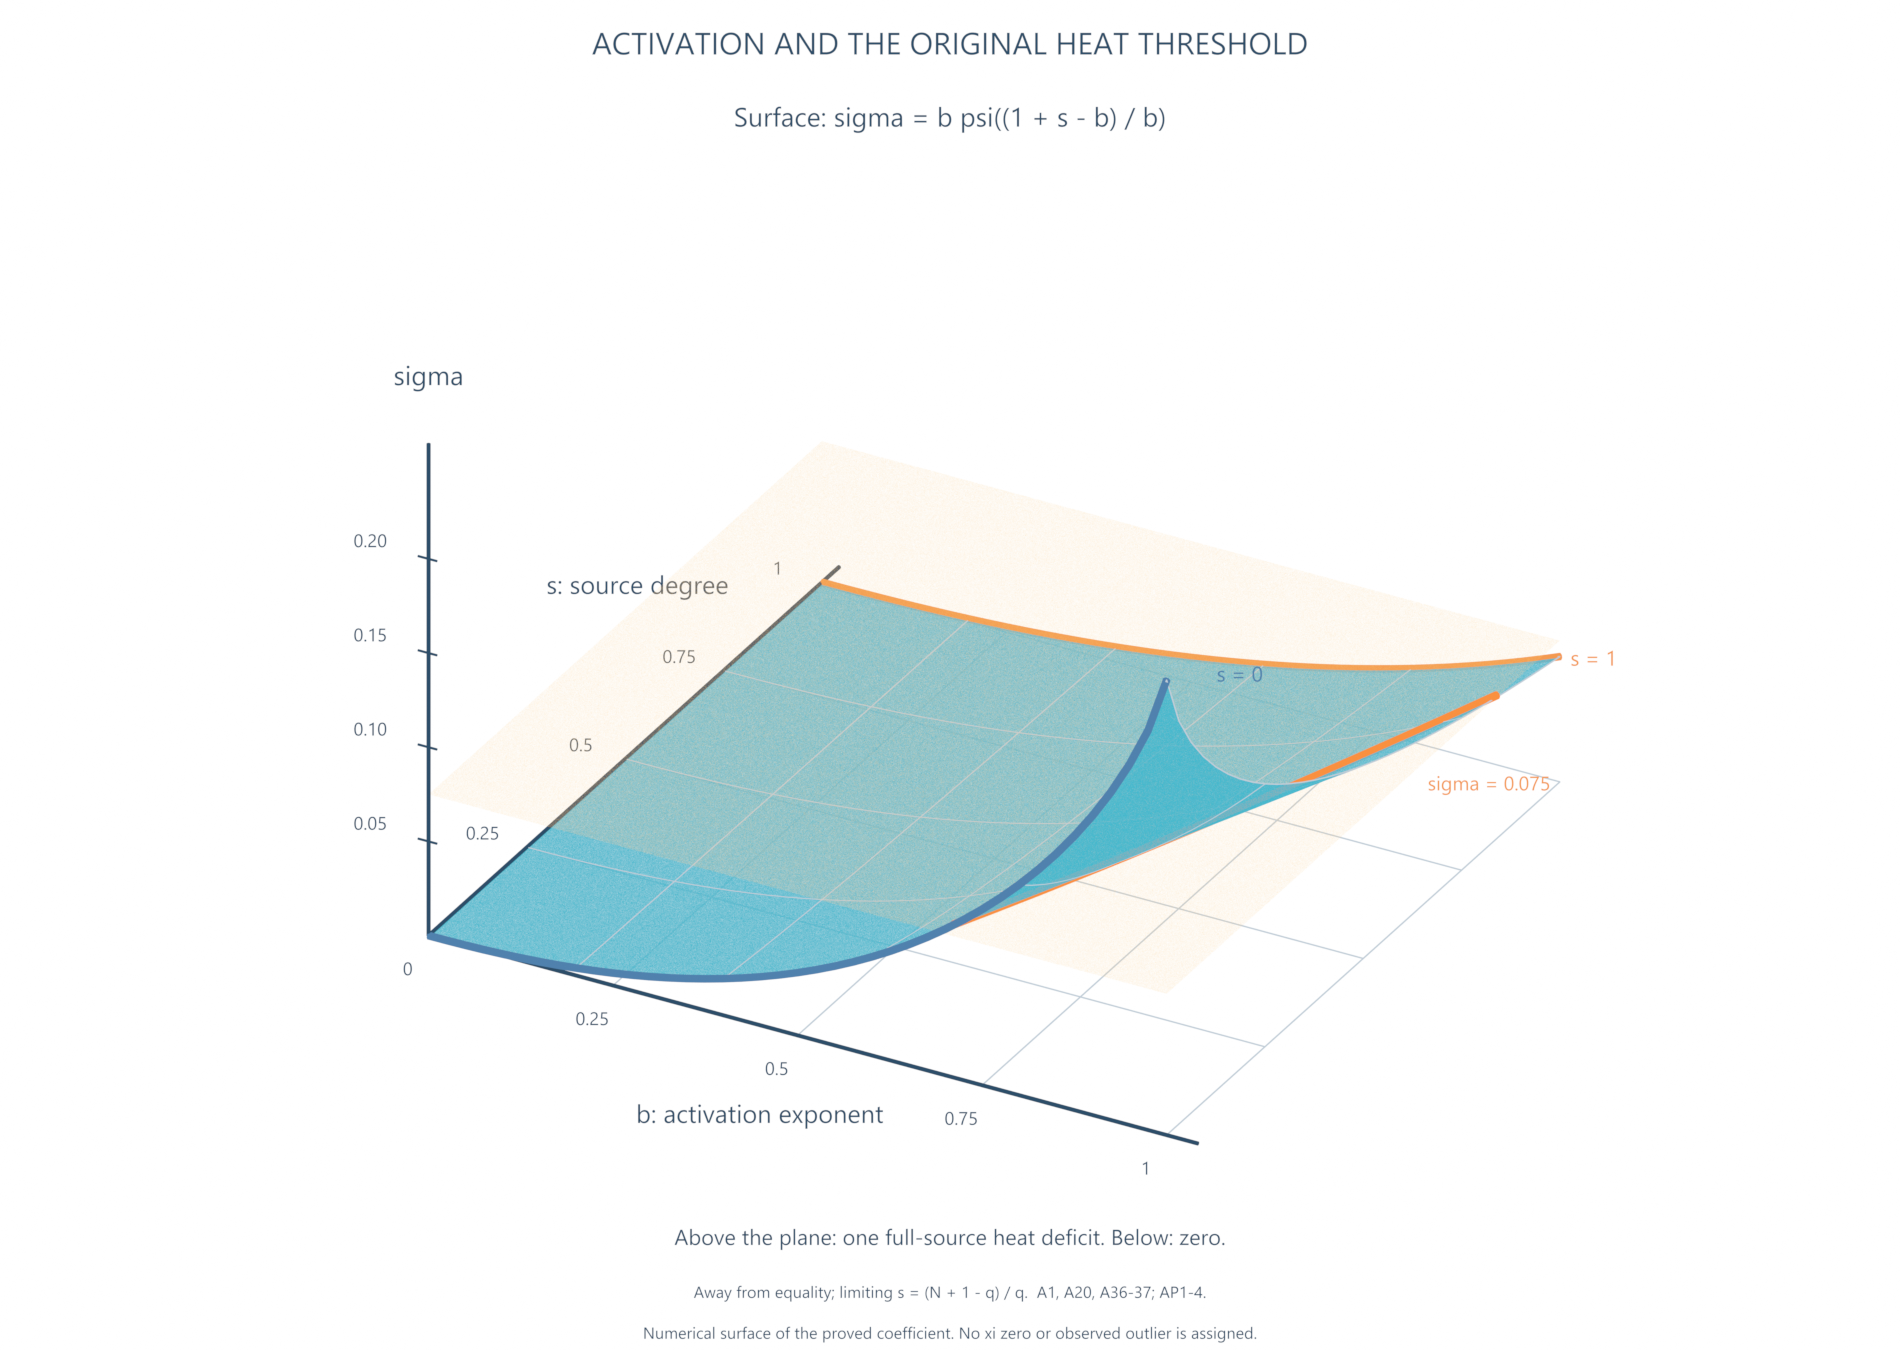
\includegraphics[width=\linewidth]{ACTIVATION_HEAT_THRESHOLD.png}
\caption{Numerical rendering of the proved fixed-activation threshold
\(\sigma=\Psi_b(s)=b\psi((1+s-b)/b)\), with \(b\in[0,1]\) and
the limiting original source coordinate \(s=(N+1-q)/q\in[0,1]\).
The displayed horizontal plane is \(\sigma=0.075\).
A surface point above it has one full-source heat deficit in A37;
a point below it has zero, away from equality. AP1--4 proves the
uniform monic estimate underlying the coefficient.
The figure assigns neither a hypothetical zeta zero nor the
observed outlier. The plotted surface uses the original elliptic
profile A20; its Gamma convention is credited to the human DLMF
authors in AP's bibliography. Scene and sample data are retained.}
\end{figure}\clearpage
\clearpage\part{The native adjacent-cutoff allocation and currents}

Adding the next orthogonal polynomial changes the original attained
quotient covariance by one column. We calculate its effect on the actual
conductor kernel and both complex projected currents. Every coefficient
of the adjacent-cutoff sign polynomial is displayed; its degree is at
most five, independent of dimension. We also prove that the two adjacent
changes of the original conductor projection determinant cost only
\(O_A(q\log(q+2))=o(kq)\). The remaining leading allocation is reduced
to the two specified original endpoints. Its value and the individual
current signs remain to be evaluated.

\section{Original source and one added column}
Use MR1--10 \cite{ACCMR}, on its complete simple-quartet five-orbit domain:
\begin{equation}\tag{ACC1}
\begin{gathered}
k\ge9,\quad k=1\pmod4,\quad q=(k+1)^2,\quad c=k/2,\\
0<\delta<1/2,\quad\gamma>2,\qquad
\lambda_{ab}=c+(2a-k)\delta+i(2b-k)\gamma,\\
\chi(S)=\prod_{a,b=0}^k(S-\lambda_{ab}),\qquad
d\mu(y)=w_h^{*k}(y)\,dy,\quad S=c+iy .
\end{gathered}
\end{equation}
Keep the original divisor \(h\), source mass, units and period.
Let \(p_j(S)\) be its monic orthogonal polynomials, with actual norms
\(\omega_j>0\). The source has finite moments and positive polynomial
Grams by MR3. The literal root-value map is \(V[P]=(P(\lambda_{ab}))\).
In these coordinates \(A=\operatorname{diag}(\lambda_{ab})\).
Keep the full invariant image \(Z=[M_A,S_kZ_k]\), its annihilator frame
\(B=\pi^T\), and \(K=\operatorname{im}B=\ker Z^T\), of dimension
\(m=8k-16\). The map from polynomial coordinates is \(I_K=V^{-1}B\).
The metrics are related by \(G=V^{-*}G^{\rm pol}V^{-1}\);
thus \(B^*GB=I_K^*G^{\rm pol}I_K\), with no change of the source.

For \(N\ge q-1\), set
\begin{equation}\tag{ACC2}
C=\sum_{j=0}^N u_ju_j^*,\qquad
(u_j)_\alpha=p_j(\lambda_\alpha)/\sqrt{\omega_j},\qquad
G=C^{-1},\qquad u=u_{N+1}.
\end{equation}
Interpolation proves \(C>0\). MR9--10 proves that \(G\) is the full
attained minimum over the entire relation ideal. The next covariance
is exactly \(C_{N+1}=C+uu^*\).
Use \(C(t)=C+tuu^*\), \(t\ge0\), to calculate this single column:
\(t=0,1\) are the original adjacent cutoffs. For \(t>0\) this is the
covariance of the source map with columns
\(u_0,\ldots,u_N,\sqrt t\,u_{N+1}\) from its displayed Euclidean
coefficient space. This specifies every intermediate source map.
The finite identities also apply separately to a specified Gamma source;
its orthogonal polynomials are not identified with the arithmetic ones.

\section{The complete allocation and moving projection}
The inverse update is the classical Sherman--Morrison identity
\cite{ACCSM}. Its needed form is proved below, with the original
source attribution retained.
All following inner products are in \(G\), conjugate-linear first.
Define
\begin{equation}\tag{ACC3}
\begin{gathered}
H=B^*GB,\quad P=BH^{-1}B^*G,\quad e=Pu,\quad f=(I-P)u,\\
a=\|e\|_G^2,\quad\beta=\|f\|_G^2,\quad\alpha=a+\beta=\|u\|_G^2,\\
d(t)=1+t\alpha,\quad b(t)=1+t\beta,\quad s(t)=t/b(t).
\end{gathered}
\end{equation}
Multiplication gives \(P^2=P\), \(P^*G=GP\), and image \(K\).
Thus \(e\perp_G f\), proving the energy equality and \(b,d\ge1\).
Multiplication by \(C+tuu^*\) proves
\begin{equation}\tag{ACC4}
G(t)=G-\frac{t}{d(t)}Guu^*G.
\end{equation}
Write \(h_B=B^*Gu\), so \(h_B^*H^{-1}h_B=a\). Direct multiplication gives
\begin{equation}\tag{ACC5}
H(t)=H-\frac{t}{d(t)}h_Bh_B^*,\qquad
H(t)^{-1}=H^{-1}+\frac{t}{b(t)}H^{-1}h_Bh_B^*H^{-1}.
\end{equation}
For invertible \(T\), expansion of \(\det(I+T^{-1}vw^*)\) by columns
has no term with two updated columns, since those columns are
proportional. Its first-order terms sum to \(w^*T^{-1}v\).
This proves \(\det(T+vw^*)/\det T=1+w^*T^{-1}v\), and hence
\begin{equation}\tag{ACC6}
\boxed{\frac{\det H(t)}{\det H}=\frac{1+t\beta}{1+t\alpha},\qquad
\frac{\det G(t)}{\det G}=\frac1{1+t\alpha}.}
\end{equation}
Choose any fixed complement \(J\) to \(B\), and let \(Q(t)\) be
the quotient minimum in its fixed quotient coordinates. It is the
Schur complement of \(H(t)\) in \([B,J]^*G(t)[B,J]\).
Block elimination gives its determinant factorization. The fixed
frame determinant cancels, proving
\begin{equation}\tag{ACC7}
\boxed{\frac{\det Q(t)}{\det Q(0)}=\frac1{1+t\beta},\qquad
-\frac{d}{dt}\log\det H(t)=
\frac{a}{(1+t\alpha)(1+t\beta)}.}
\end{equation}
The kernel loss in one original step is
\(\log((1+\alpha)/(1+\beta))\); the complementary loss is
\(\log(1+\beta)\). Both use the actual projected column.

Substituting ACC4--5 in \(BH(t)^{-1}B^*G(t)\) gives
\begin{equation}\tag{ACC8}
\boxed{P(t)=P-\frac{t}{1+t\beta}e f^*G.}
\end{equation}
Indeed the coefficient of \(e u^*G\) is
\(-t/d-t^2a/(bd)=-t/b\), and the other added term is
\(t e u^*GP/b\). This verifies the formula while retaining
the original moving projection.

\begin{figure}[ht]\centering
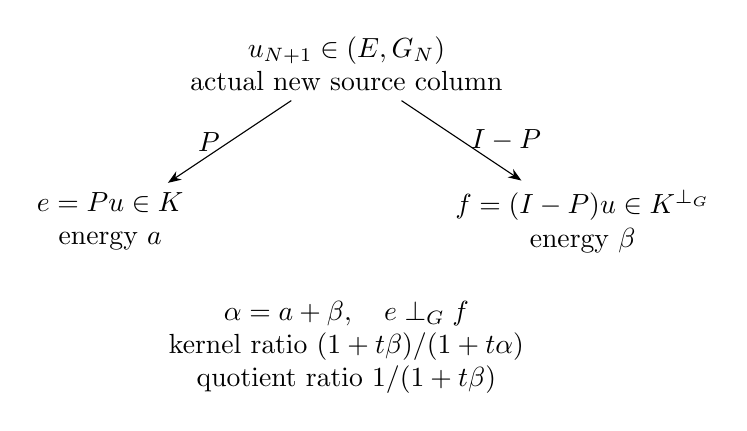
\begin{tikzpicture}[>=Stealth,every node/.style={align=center}]
\node (u) at (0,0) {$u_{N+1}\in(E,G_N)$\\actual new source column};
\node (e) at (-3,-2) {$e=Pu\in K$\\energy \(a\)};
\node (f) at (3,-2) {$f=(I-P)u\in K^{\perp_G}$\\energy \(\beta\)};
\draw[->] (u)--node[left] {\(P\)}(e);
\draw[->] (u)--node[right] {\(I-P\)}(f);
\node at (0,-3.6) {\(\alpha=a+\beta,\quad e\perp_G f\)\\
kernel ratio \((1+t\beta)/(1+t\alpha)\)\\
quotient ratio \(1/(1+t\beta)\)};
\end{tikzpicture}
\caption{Exact maps and energies ACC3--7. The kernel annihilates the
complete original invariant image. No angle or numerical energy is
assigned by the drawing. MR9 supplies the orthogonal-polynomial
source column, with its original human-source citations.}
\end{figure}

\section{Every coefficient of both complex currents}
Fix any original physical class \(x\), without altering its norm.
This includes the actual root eigenclasses. Put
\begin{equation}\tag{ACC9}
p=Px,\quad o=(I-P)x,\quad \rho=f^*Gx=\ip f o,\quad
p_1=\beta p-\rho e,\quad o_1=\beta o+\rho e.
\end{equation}
Then \(P(t)x=(p+tp_1)/b(t)\) and
\((I-P(t))x=(o+to_1)/b(t)\).
Keep the complete arithmetic action in
\begin{equation}\tag{ACC10}
z(t)=\langle P(t)x,A(I-P(t))x\rangle_{G(t)},\qquad
w(t)=\langle(I-P(t))x,AP(t)x\rangle_{G(t)} .
\end{equation}
Define the following actual contractions:
\begin{equation}\tag{ACC11}
\begin{aligned}
J_0&=\ip p{Ao},&
J_1&=\ip{p_1}{Ao}+\ip p{Ao_1},&
J_2&=\ip{p_1}{Ao_1},\\
T_0&=\ip p u\,\ip u{Ao},\\
T_1&=\ip{p_1}u\,\ip u{Ao}+\ip p u\,\ip u{Ao_1},\\
T_2&=\ip{p_1}u\,\ip u{Ao_1}.
\end{aligned}
\end{equation}
All four coefficients of the first numerator are
\begin{equation}\tag{ACC12}
Z_0=J_0,\quad Z_1=J_1+\alpha J_0-T_0,\quad
Z_2=J_2+\alpha J_1-T_1,\quad Z_3=\alpha J_2-T_2 .
\end{equation}
For the second define
\begin{equation}\tag{ACC13}
\begin{gathered}
w_0=\ip o{Ap},\quad
L=\rho\ip o{Ae}+\overline\rho\ip f{Ap},\quad
T_f=|\rho|^2\ip f{Ae},\\
W_0=w_0,\qquad W_1=2\beta w_0-L,\qquad
W_2=\beta^2w_0-\beta L+T_f .
\end{gathered}
\end{equation}
Then the exact complex currents on the whole path are
\begin{equation}\tag{ACC14}
\boxed{z(t)=\frac{\sum_{j=0}^3Z_jt^j}{d(t)b(t)^2},\qquad
w(t)=\frac{\sum_{j=0}^2W_jt^j}{b(t)^2}.}
\end{equation}
To prove this, substitute ACC4 and ACC9 into the first current.
Its numerator is
\(d\ip{p+tp_1}{A(o+to_1)}
-t\ip{p+tp_1}u\ip u{A(o+to_1)}\), which expands to ACC12.
For the second, use \(o+s\rho e\) and \(p-s\rho e\).
Their metric correction contains
\(\langle o+s\rho e,u\rangle_G
=\overline\rho(1+sa)=\overline\rho\,d/b\).
Combining it with the four uncorrected pairing terms gives
\(w=w_0-sL+s^2T_f\). Multiplication by \(b^2\) proves ACC13--14.

The following six real numbers retain all complex phases:
\begin{equation}\tag{ACC15}
\begin{aligned}
r_0&=\Re(\overline Z_0W_0),\\
r_1&=\Re(\overline Z_0W_1+\overline Z_1W_0),\\
r_2&=\Re(\overline Z_0W_2+\overline Z_1W_1+\overline Z_2W_0),\\
r_3&=\Re(\overline Z_1W_2+\overline Z_2W_1+\overline Z_3W_0),\\
r_4&=\Re(\overline Z_2W_2+\overline Z_3W_1),\\
r_5&=\Re(\overline Z_3W_2).
\end{aligned}
\end{equation}
Consequently
\begin{equation}\tag{ACC16}
\boxed{\Re(\overline{z(t)}w(t))
=\frac{\sum_{j=0}^5r_jt^j}{(1+t\alpha)(1+t\beta)^4}.}
\end{equation}
The old endpoint equals \(r_0\); the new endpoint equals
\(\sum_jr_j/((1+\alpha)(1+\beta)^4)\).
A nonzero numerator has at most five positive zeros counted with
multiplicity. If all six coefficients vanish, the current is zero
on the whole path. This covers every degenerate case.
In particular \(f=0\) gives \(\beta=\rho=0\), a constant \(w\) and
a linear numerator for \(z\). If \(u=0\), everything is unchanged.
The finite coefficients specialize the earlier full-current formulas
to the actual source step. Their values still depend on the original
period, class and arithmetic metric; no sign is inferred from volume
monotonicity or from replacing that metric by Gamma.

\section{The adjacent changes of the original projection determinant}
Use the separate lower Gamma source of CGR and CGS \cite{ACCCGR,ACCCGS},
with their exact \(v,c',q',g\) and the same invariant row frame
\(R_Z>0\) at all four cutoffs. Put
\(D=N-v\), \(M=D-q'\), and \(I_N=\chi'\mathcal P'_M\subset\mathcal P'_D\).
The fixed functional for a row \(z\) is
\(\ell_z[P]=[P(\partial_w)G_z(w)]_{w=0}\), with \(G_z=F_z/E_A\).
Polynomial evaluation here uses the original \(S'\) coordinate.
Let \(C_N^U\) be the Gram of these functionals restricted to \(I_N\),
and \(\widetilde C_N\) their Gram on \(\mathcal P'_D\).
Then \(S_N=\widetilde C_N^{-1/2}C_N^U\widetilde C_N^{-1/2}>0\).

There is exactly one orthogonal new direction in each nested
inclusion \(I_N\subset I_{N+1}\), \(\mathcal P'_D\subset\mathcal P'_{D+1}\).
To specify it, form the monic degree-\(M+1\) orthogonal polynomial
\(\psi_{M+1}\) for
\(|\chi'(c'+iy)|^2d\sigma(y)\) on \(S'=c'+iy\), with norm
\(\nu_{M+1}\). All its moments are finite and its Gram is positive.
Then \(\chi'\psi_{M+1}/\sqrt{\nu_{M+1}}\) is the unit complement to
\(I_N\). Let \(\phi_{D+1,c'}\) be the original unit Gamma polynomial.
Define
\(a_N=(\ell_z[\chi'\psi_{M+1}]/\sqrt{\nu_{M+1}})_z\) and
\(b_N=(\ell_z[\phi_{D+1,c'}])_z\).
The two orthogonal decompositions give exactly
\begin{equation}\tag{ACC17}
C_{N+1}^U=C_N^U+a_Na_N^*,\qquad
\widetilde C_{N+1}=\widetilde C_N+b_Nb_N^* .
\end{equation}
These are the same fixed functionals on nested full lower-root ideals.
The determinant identity proved above gives
\begin{equation}\tag{ACC18}
\log\det S_{N+1}-\log\det S_N
=\log(1+a_N^*(C_N^U)^{-1}a_N)
-\log(1+b_N^*\widetilde C_N^{-1}b_N).
\end{equation}
Use the complete finite bounds CGR15 and CGS14--15:
\begin{equation}\tag{ACC19}
\begin{gathered}
l_NR_Z\preceq C_N^U\preceq u_NR_Z,\qquad
\widetilde l_NR_Z\preceq\widetilde C_N\preceq u_NR_Z,\\
l_N=(M_D^2B_{\rm val}qC_A^{2q'})^{-1},\quad
\widetilde l_N=(M_D^2B_E)^{-1},\quad
u_N=V_NM_D^{2D}e^{2J_D}.
\end{gathered}
\end{equation}
The constants are those defined and proved in those complete sources.
Every logarithmic allowance is \(O_A(q\log(q+2))\).
If \(C'=C+aa^*\), all eigenvalues of \(C^{-1/2}C'C^{-1/2}\)
are one except \(1+a^*C^{-1}a\). The bounds \(C\succeq lR\),
\(C'\preceq uR\) imply that last eigenvalue is at most \(u/l\).
Thus, with \(\log^+s=\max(0,\log s)\),
\begin{equation}\tag{ACC20}
\begin{gathered}
0\le\log(1+a_N^*(C_N^U)^{-1}a_N)\le A_N:=\log^+(u_{N+1}/l_N),\\
0\le\log(1+b_N^*\widetilde C_N^{-1}b_N)
\le B_N:=\log^+(u_{N+1}/\widetilde l_N),\\
-B_N\le\delta_N:=\log\det S_{N+1}-\log\det S_N\le A_N .
\end{gathered}
\end{equation}
There is no full-row-rank multiplier: only one eigenvalue changes.
Keeping all four signs proves
\begin{equation}\tag{ACC21}
\begin{aligned}
&\log\frac{\det S_{q-1}\det S_q}{\det S_{2q-1}\det S_{2q}}
=2\log\frac{\det S_{q-1}}{\det S_{2q-1}}
+\delta_{q-1}-\delta_{2q-1},\\
&|\delta_{q-1}-\delta_{2q-1}|
\le E_{\rm adj}:=\max(A_{q-1},B_{q-1})
+\max(A_{2q-1},B_{2q-1})=o_A(kq).
\end{aligned}
\end{equation}
The two adjacent endpoints are retained in the exact correction.

With the full finite error \(E_{\rm DCR}\) of DCR26 \cite{ACCDCR},
\(g=16k-48-v\), and
\(\mathcal Rf=f_{q-1}+f_q-f_{2q-1}-f_{2q}\), this yields
\begin{equation}\tag{ACC22}
\boxed{\left|\mathcal R\log\det H_{K,N}^{\rm ar}
-gq\mathfrak C_\partial
-2\log\frac{\det S_{q-1}}{\det S_{2q-1}}\right|
\le E_{\rm DCR}+E_{\rm adj}=o_{A,h}(kq).}
\end{equation}
For \(k\ge17\), CGP24--27 \cite{ACCCGP} gives the two finite sampled
ratios \(\mathcal A_N^{[T]}\), on its actual pole-canceling rows,
with errors \(P_N+2t_k\log(4/3)\).
Substitution only at these two endpoints proves
\begin{equation}\tag{ACC23}
\begin{aligned}
&\left|\mathcal R\log\det S_N
-2(\mathcal A_{q-1}^{[T]}-\mathcal A_{2q-1}^{[T]})\right|\\
&\quad\le E_{\rm adj}+2(P_{q-1}+P_{2q-1})+8t_k\log(4/3)=o_A(kq).
\end{aligned}
\end{equation}
The sample counts and complementary row costs remain the explicit
CGP20/27 constants. No sampled value or leading coefficient is
presumed computed.

\section{The new activated source: both added columns and their interference}
The new supplied activation proof \cite{ACCActivation}, A28--30, uses the
same fixed tensor section \(Y\) at every cutoff. We verify its exact
receiver here. The scalar source inclusion \(X_N\subset X_{N+1}\)
adds its orthonormal polynomial \(\phi_{N+1}\).
The joint inclusion \(X_N+Y\subset X_{N+1}+Y\) adds the orthogonal
residual \(z=(I-P_{X_N+Y})\phi_{N+1}\). If it is nonzero, divide it
by its physical norm; if it is zero the new column is zero.
Let \(f_N,g_N\) be their respective values in the original quotient.
Every vector of zero value is still part of the physical minimum.
The orthogonal decompositions give, at fixed \(0\le\eta\le1\),
\begin{equation}\tag{ACC24}
C_{N+1}(\eta)=C_N(\eta)+UU^*,\quad
U=[\,\sqrt{1-\eta}\,f_N,\ \sqrt\eta\,g_N\,],\quad
C_N(\eta)=(1-\eta)G_N^{-1}+\eta(G_N^J)^{-1}.
\end{equation}
The symbol \(\eta\) in this section means the source activation only.

The following calculation also covers zero or dependent columns.
Use \(G=C_N(\eta)^{-1}\) and its full original kernel projection \(P\).
For \(U\) having \(d_s\) columns (\(d_s=2\) in ACC24), set
\[
E=PU,\quad F=(I-P)U,\quad
\mathsf A=U^*GU,\quad\mathsf B=F^*GF,\quad
D(t)=I+t\mathsf A,\quad B(t)=I+t\mathsf B.
\]
Both small matrices are positive definite for \(t\ge0\).
Their determinants are denoted \(d(t)\) and \(b(t)\). Direct
multiplication verifies
\begin{equation}\tag{ACC25}
G(t)=G-tGU D(t)^{-1}U^*G,\qquad
P(t)=P-tE B(t)^{-1}F^*G.
\end{equation}
For completeness, put \(H=B_K^*GB_K\) for any fixed kernel frame,
and \(L=B_K^*GU\). Then \(L^*H^{-1}L=E^*GE=\mathsf A-\mathsf B\).
Multiplication proves
\(H(t)^{-1}=H^{-1}+tH^{-1}L B(t)^{-1}L^*H^{-1}\);
substituting it into the kernel projection gives ACC25.
Block elimination of
\(\left(\begin{smallmatrix}I&X\\-Y&I\end{smallmatrix}\right)\)
in either order gives \(\det(I+XY)=\det(I+YX)\).
This proves the exact determinant allocations
\begin{equation}\tag{ACC26}
\frac{\det H(t)}{\det H}=\frac{b(t)}{d(t)},\qquad
\frac{\det Q(t)}{\det Q(0)}=\frac1{b(t)}.
\end{equation}
For the actual two columns,
\begin{equation}\tag{ACC27}
\begin{aligned}
d(t)&=1+t\,\operatorname{Tr}\mathsf A
+t^2(\mathsf A_{11}\mathsf A_{22}-|\mathsf A_{12}|^2),\\
b(t)&=1+t\,\operatorname{Tr}\mathsf B
+t^2(\mathsf B_{11}\mathsf B_{22}-|\mathsf B_{12}|^2).
\end{aligned}
\end{equation}
Both complex interference terms remain. In particular the full
activated kernel loss is exactly \(\log d(1)-\log b(1)\).

There is also an explicit finite polynomial for its original current.
For the unchanged physical class \(x\), put \(p=Px\), \(o=(I-P)x\),
\(\rho=F^*Gx\), and
\[
\Delta(t)=\operatorname{adj}D(t),\quad
\mathcal B(t)=\operatorname{adj}B(t),\quad
v(t)=b(t)p-tE\mathcal B(t)\rho,\quad
w_s(t)=b(t)o+tE\mathcal B(t)\rho .
\]
Define the two scalar polynomials
\begin{equation}\tag{ACC28}
\begin{aligned}
Z(t)&=v(t)^*[d(t)G-tGU\Delta(t)U^*G]A w_s(t),\\
W(t)&=[b(t)o^*G-t\rho^*\mathcal B(t)F^*G]A v(t).
\end{aligned}
\end{equation}
Conjugation here acts on coefficients with real \(t\).
Then the two currents ACC10 satisfy exactly
\begin{equation}\tag{ACC29}
z(t)=\frac{Z(t)}{d(t)b(t)^2},\qquad
w(t)=\frac{W(t)}{b(t)^2},\qquad
\Re(\overline zw)=\frac{\Re(\overline{Z(t)}W(t))}{d(t)b(t)^4}.
\end{equation}
To check the cancellation in the second formula, write
\(o_t=o+tEB(t)^{-1}\rho\).
Since \(U^*Go_t=D(t)B(t)^{-1}\rho\), ACC25 gives
\(o_t^*G(t)=o^*G-t\rho^*B(t)^{-1}F^*G\).
The first formula is direct substitution. Thus every factor and
both moving projections are accounted for.

The adjugates have degree at most \(d_s-1\).
Hence \(v,w_s\) have degree at most \(d_s\), the bracket defining
\(Z\) has degree at most \(d_s\), and
\[
\deg Z\le3d_s,\quad \deg W\le2d_s,\quad
\deg\Re(\overline ZW)\le5d_s.
\]
For the new activated adjacent cutoffs this is degree at most ten.
Its endpoint is obtained by \(t=1\) in ACC28--29, with exactly
the original \(U\) of ACC24. This supplies the missing fixed-kernel
and complex-current receivers of the two-column covariance
calculation. It does not assign those native phases from its
\(q^2\) determinant coefficient.

\begin{thebibliography}{9}
\bibitem{ACCSM} J. Sherman and W. J. Morrison,
\emph{Adjustment of an Inverse Matrix Corresponding to a Change
in One Element of a Given Matrix}, Annals of Mathematical Statistics
21 (1950), 124--127,
\href{https://doi.org/10.1214/aoms/1177729893}{doi:10.1214/aoms/1177729893}.
\bibitem{ACCActivation} Supplied web-session derivation,
\emph{The actual outgoing polynomial under source activation},
A1--38, received 21 September 2026. The complete source is retained
with this continuation; human authorship is unspecified in that source.
\bibitem{ACCMR} Split-Zero research programme,
\emph{The original observation kernel as an exact mixed-relation
determinant}, MR1--10.
\href{https://github.com/KokunoYumeto/zeta-function-research-reader/blob/5992ad50c0f2a06921f1fcaded7b4e38097c0739/workbenches/splitzero-tandem/continuations/20260920-original-kernel-mixed-determinants/ORIGINAL_KERNEL_MIXED_DETERMINANT.tex#L36}{Complete pinned public proof}.
\bibitem{ACCCGR} Split-Zero research programme,
\emph{The original covariance and its conductor-pole filtration},
CGR13--17, complete source supplied with this continuation.
\bibitem{ACCCGS} Split-Zero research programme,
\emph{The original strip and its projection-angle loss},
CGS13--22, complete source supplied with this continuation.
\bibitem{ACCDCR} Split-Zero research programme,
\emph{The evaluated outer return and the actual arithmetic kernel},
DCR1--27, especially DCR26, complete source supplied with this continuation.
\bibitem{ACCCGP} Split-Zero research programme,
\emph{The original lower-root projection: exact action, zero kernel,
and a finite determinant formula with \(o(kq)\) error},
CGP1--28, reproduced completely in the reader.
\bibitem{ACCDLMF} T. H. Koornwinder, R. Wong, R. Koekoek,
R. F. Swarttouw, with W. P. Reinhardt,
\emph{Orthogonal Polynomials}, Chapter 18 of the
NIST Digital Library of Mathematical Functions,
F. W. J. Olver et al., editors,
\url{https://dlmf.nist.gov/18.22.E8} and
\url{https://dlmf.nist.gov/18.23.E7}.
The original-author TeX recurrence and generating-function encodings
are retained in the source ledger. Their exact Gamma specialization is
proved in the accompanying CG and CGP sources. Every inverse, projection,
determinant and current identity needed above is proved directly here.
\end{thebibliography}
\clearpage\part{Uniform monic control and native receiving estimates}

This note supplies the uniform monic-norm estimate used in A19 of the
new activation proof \cite{APActivation}. It also gives explicit source
comparison bounds sufficient for that proof's action and observation
receivers. The original finite Taylor-to-\(Q\) return, the full tensor
section and its physical normal source remain those in A6--18.
This argument evaluates the fixed-activation \(q^2\) law. It does not
supply the smaller error required for the canonical \(kq\) allocation.

\section{The exact equilibrium family and uniform constants}
Let \(t\) range over a fixed compact interval
\(J=[t_-,t_+]\subset(0,\infty)\), and set
\[
V_t(x)=\frac{\pi}{t}\sqrt x-\frac2t\log x.
\]
EIQ1--19 \cite{APEIQ} proves directly its equilibrium probability
\(\mu_t\), supported on \([a_t,b_t]\), with
\[
V_t(x)-2\int\log|x-y|\,d\mu_t(y)=\lambda_t
\quad(a_t\le x\le b_t),
\]
and a larger value outside that interval in \((0,\infty)\).
The density is EIQ10--11:
\[
\frac{\sqrt{(b_t-x)(x-a_t)}}{2\pi}
\frac{\beta_t}{2\pi x}
\int_0^\infty
\frac{\sqrt s\,ds}{(x+s)\sqrt{(a_t+s)(b_t+s)}},
\qquad \beta_t=\pi/t.
\]
Its endpoints depend smoothly on \(t\), by EIQ3--6.
Consequently \(a_*=\min_Ja_t>0\),
\(b^*=\max_Jb_t<\infty\), and \(\min_J(b_t-a_t)>0\).
The displayed integral, split at \(s=1\), is uniformly bounded:
near zero its integrand is at most a constant times \(\sqrt s\);
near infinity it is at most a constant times \(s^{-3/2}\).
The density therefore has a uniform upper bound \(M_J\).
The same formulas give a bounded continuous \(\lambda_t\).
These are proved properties of this specified family, rather than
regularity assumptions about an arbitrary equilibrium measure.

For \(\epsilon\in\{0,1\}\), put
\[
w_{t,\epsilon}(x)
=x^{\epsilon+\epsilon/t-3/4}
 e^{-\pi\epsilon\sqrt x/(2t)} .
\]
On every equilibrium interval this function and its reciprocal
are uniformly bounded. On \((0,B]\), for fixed \(B\), it is
uniformly integrable, since its smallest exponent at zero is
\(-3/4>-1\).

\section{A complete uniform monic-norm bound}
For a positive integer \(h\), define
\[
I_h(t,\epsilon)=
\min_{\substack{P\ {\rm monic}\\\deg P=h}}
\int_0^\infty |P(x)|^2e^{-hV_t(x)}w_{t,\epsilon}(x)\,dx.
\]
We prove constants \(c_J,C_J,L_J>0\) such that
\begin{equation}\tag{AP1}
c_Je^{-h\lambda_t}\le I_h(t,\epsilon)
\le C_J(h+2)^{L_J}e^{-h\lambda_t}.
\end{equation}

For the lower bound let \(\omega_t\) be the arcsine probability on
\([a_t,b_t]\), and \({\rm cap}_t=(b_t-a_t)/4\).
For every complex \(z\),
\[
\int\log|x-z|\,d\omega_t(x)\ge\log{\rm cap}_t .
\]
To verify this, write \(x=(a_t+b_t)/2+(b_t-a_t)\cos\theta/2\).
Factor \(x-z\) into its two reciprocal factors in \(e^{i\theta}\).
The mean of \(\log|e^{i\theta}-w|\) is
\(\log\max(1,|w|)\): for \(|w|<1\) expand
\(\log(1-we^{-i\theta})\) and integrate its real part; for
\(|w|>1\) factor out \(w\); at \(|w|=1\) take the integrable
logarithmic limit. The resulting additional term is nonnegative,
proving the assertion, with equality for \(z\) in the interval.
Apply it to every zero of \(P\).
Jensen's inequality on the interval gives
\[
\begin{split}
\log\int |P|^2e^{-hV_t}w_{t,\epsilon}\,dx
&\ge 2h\log{\rm cap}_t-h\int V_t\,d\omega_t\\
&\quad+\int\log(w_{t,\epsilon}/\omega_t')\,d\omega_t .
\end{split}
\]
The final integral is uniformly bounded below. Indeed \(w\) is
bounded above and below there, and the arcsine logarithmic
singularities are integrable, uniformly for the stated interval
lengths. Averaging the exact EIQ Euler equality against \(\omega_t\)
and interchanging the integrable logarithmic kernels gives
\[
\int V_t\,d\omega_t-2\log{\rm cap}_t=\lambda_t.
\]
The lower bound in AP1 follows. A root of \(P\) on the interval
causes an integrable logarithm; Jensen follows by a positive
regularization and its limit.

For the upper bound take the \(h\) midpoint quantiles \(x_j\) of
\(\mu_t\), and \(P_h(x)=\prod_{j=1}^h(x-x_j)\).
The empirical distribution \(\mu_{t,h}\) satisfies
\(\sup_x|\mu_{t,h}((-\infty,x])-\mu_t((-\infty,x])|
\le1/(2h)\). Fix a finite \(B>b^*+1\), and put
\(\varepsilon_h=1/h\) and
\(f_x(y)=\log\max(|x-y|,\varepsilon_h)\).
For \(x\in[0,B]\) its total variation on the support is at most
\(C_{J,B}+2\log(h+2)\): it decreases toward the truncated
minimum and then increases, and its maximum is bounded by
\(\log(B+b^*+1)\).
Integration by parts for a bounded-variation function against the
difference of the two distribution functions therefore gives
\[
\left|\int f_x\,d(\mu_{t,h}-\mu_t)\right|
\le\frac{C_{J,B}+2\log(h+2)}{2h}.
\]
The density bound proves
\[
0\le\int(f_x(y)-\log|x-y|)\,d\mu_t(y)
\le 2M_J\varepsilon_h,
\]
because \(\int_0^\varepsilon\log(\varepsilon/u)\,du=\varepsilon\).
Since the untruncated discrete logarithm is at most the truncated
one, these two estimates give uniformly on \([0,B]\)
\[
\log|P_h(x)|
\le h\int\log|x-y|\,d\mu_t(y)+C_J\log(h+2).
\]
The full Euler inequality then bounds its squared weighted
integrand by
\((h+2)^{C_J}e^{-h\lambda_t}w_{t,\epsilon}(x)\).
Its integral on \([0,B]\) has the claimed upper bound.

Choose \(B>2b^*\) large enough that, for all \(x\ge B\) and \(t\in J\),
\[
(2+2/t)\log x-(\pi/t)\sqrt x
\le-\lambda_t-c\sqrt x,\qquad c=\pi/(2t_+)>0 .
\]
Such a common \(B\) exists since \(\log x/\sqrt x\to0\) and
\(\lambda_t\) is bounded. One can choose it by imposing the
inequality at \(B\) and
\(\sqrt B\ge 2(2+2/t_-)/c\), which makes its sufficient envelope
decrease thereafter. All the polynomial zeros lie in \((0,b^*]\);
hence \(|P_h(x)|\le x^h\) for \(x\ge B\).
The tail is bounded by
\[
e^{-h\lambda_t}\int_B^\infty
 x^{\,1+1/t_-}e^{-hc\sqrt x}\,dx
\le C_Je^{-h\lambda_t}.
\]
Here the exponent also bounds the possible negative power on this
interval. This proves the upper half of AP1, including both
integration regions. No uniform lower density bound at the soft
edges was required.

\section{Return to the exact Gamma and arithmetic monic minima}
Use the complete Gamma measure
\(d\sigma(y)=|\Gamma(1/4+iy/2)|^2dy/(2\pi)\),
with mass \(M_\sigma=\sqrt{2\pi}\), recurrence and norms
\[
p_{j+1}=yp_j-j(j-\tfrac12)p_{j-1},\qquad
\gamma_j=M_\sigma j!(1/2)_j .
\]
Their original-source citations and full constant conventions are
in CG4/8 and DLMF \cite{APCG,APDLMF}.
Let \(n=L+r\), \(r=2h+\epsilon\), and \(t=r/L\in J\).
Because the weight \(|y|^{2L}d\sigma\) is even, its unique monic
minimizer has parity \(r\). Uniqueness follows from its positive
Gram; reflection is another minimizer, so they coincide.
Write it as \(U_r(y)=y^\epsilon V_h(y^2)\).
The exact substitution \(y=L\sqrt x\), including both real
half-lines, yields
\[
\int_{\mathbb R}|y|^{2L}|U_r(y)|^2d\sigma(y)
=L^{2n+1}\int_0^\infty x^{L+\epsilon-1/2}
 |\widehat V_h(x)|^2\,\sigma(L\sqrt x)\,dx,
\]
where \(\widehat V_h(x)=L^{-2h}V_h(L^2x)\) is monic.
Here the required density bounds follow directly from Binet's formula
of Askey and Roy \cite{APBinet}, whose original TeX accompanies this edition.
For $\Re z>0$ it states
\[
\log\Gamma(z)=(z-\tfrac12)\log z-z+\tfrac12\log(2\pi)+R(z),\quad
R(z)=\int_0^\infty e^{-zs}
\left(\frac1{e^s-1}-\frac1s+\frac12\right)\frac{ds}{s}.
\]
For $u>0$, differentiation gives $u\cosh u-\sinh u\ge0$.
The coefficient of $u^{2j+1}$ in
$(1+u^2/3)\sinh u-u\cosh u$ is
$4j(j-1)/(3(2j+1)!)\ge0$. Thus
$0\le\coth u-u^{-1}\le u/3$, and consequently
\[
0\le\frac1{e^s-1}-\frac1s+\frac12\le s/12,\qquad
|R(z)|\le(12\Re z)^{-1}.
\]
Put $Y=|y|/2$, $a=1/4$, $r_Y=(a^2+Y^2)^{1/2}$.
Twice the real part, with the original $2\pi$ removed, gives
\[
\log\sigma(y)+\tfrac12\log Y+\pi Y
=-\tfrac12\log(r_Y/Y)+2Y\arctan(a/Y)-\tfrac12
 +2\Re R(a+iY).
\]
This is at most $2/3$, since $\arctan v\le v$.
For $Y\ge1/2$, it is at least
$-7/6-\tfrac14\log(5/4)$, since $r_Y/Y\le\sqrt{5/4}$.
Therefore, with the explicit constants
$C_U=\sqrt2e^{2/3}$ and
$C_L=\sqrt2e^{-7/6}(5/4)^{-1/4}$, the bounds are
\(\sigma(y)\le C_U|y|^{-1/2}e^{-\pi|y|/2}\) for \(y\ne0\),
and the corresponding positive lower bound with \(C_L\) for
\(|y|\ge1\). Thus the prefactor is \(L^{2n+1/2}\).
The exact remaining weight factors as
\[
x^{L+\epsilon-3/4}e^{-\pi L\sqrt x/2}
=e^{-hV_t(x)}w_{t,\epsilon}(x).
\]
The global upper bound and AP1's explicit trial give the upper
monic estimate. The lower density bound holds on the equilibrium
interval once \(L\sqrt{a_*}\ge1\); AP1's interval-only lower proof
then applies. It follows that
\begin{equation}\tag{AP2}
\log\nu_r^{(L),\Gamma}
=(2n+\tfrac12)\log L-h\lambda_t+O_J(\log(h+2)).
\end{equation}
The finitely many smaller integral pairs can be retained in the
constant. This also proves that no zero neighborhood was removed
from the upper integral.

The exact factorial norm gives
\(\log\gamma_n=2n\log n-2n+O(\log(n+2))\).
Using \(n=L(1+t)\) and \(h=(Lt-\epsilon)/2\) in AP2 gives
\begin{equation}\tag{AP3}
\log\frac{\nu_r^{(L),\Gamma}}{\gamma_n}
=2L\psi(t)+O_J(\log(n+2)),\quad
\psi(t)=(1+t)(1-\log(1+t))-\frac t4\lambda_t .
\end{equation}
This is the original profile, with the full source mass canceled
only in the displayed ratio.

For the arithmetic source, A8's proved polynomial form bounds
apply to every polynomial \(y^LU_r\) as well as to every degree-\(n\)
monic polynomial. Taking their two separate minima gives
\[
\left|\log\frac{\nu_r^{(L),\mu}}{\omega_n^\mu}
-\log\frac{\nu_r^{(L),\Gamma}}{\gamma_n}\right|
\le\log(c_+/c_-).
\]
There is no determinant rank factor. The earlier profile is
positive on finite positive \(t\), with a positive minimum on \(J\).
For \(L\) proportional to \(q\), the last error is
\(O_h(k\log^2(q+2))=o(q)\); subtracting one from the ratio has
exponentially small relative effect. Therefore the actual
Taylor minimum A12 satisfies
\begin{equation}\tag{AP4}
\log J_{n,L}=L\psi((n-L)/L)
+O_{h,J}(k\log^2(q+2)+\log(q+2)).
\end{equation}
This proves the uniform estimate needed in A19 on exactly its
fixed compact parameter domain.

\section{The original action and observation estimates}
A8 alone gives a sufficient compression bound without needing a
linear-in-\(q\) arithmetic recurrence estimate. If \(T_N\) is the
actual attained scalar minimum section, then its real multiplication
compression satisfies
\begin{equation}\tag{AP5}
\|T_N^*yT_N\|_\mu
\le (2N+3)\sqrt{c_+/c_-}=e^{o_h(q)}
\end{equation}
through the admitted window. The earlier complete-source theorem
NG3 \cite{APNG} also proves the sharper bound
\(C_{\rm mult}(h)(2N+\lfloor k/3\rfloor)=O_h(q)\);
its original outgoing degree face is included in that proof.
Thus the incoming A23 linear bound remains available.
For the independent bound AP5, the Gamma Jacobi off-diagonal
coefficients are \(\sqrt{j(j-1/2)}\), so multiplication through degree
\(N\) has norm at most \(2N+3\). Apply A8 to \(yP\) and \(P\), and
then use that the minimum section is an isometry and its adjoint
contracts. This explicit alternative also suffices for A24--27 and
the entire subcritical heat conclusion.

The original observation admits a stronger finite comparison. Keep
the full degree-$q$ relation $Q$, with root radius $R$ and every
multiplicity, and the guards $q\ge8$, $R/q\le1/2$.
Put $\widehat Q(w)=q^{-q}Q(qw)$. The coordinate map is
$p(y)\mapsto p(qw)$; the physical norm is kept throughout.
For any degree-$N$ polynomial $F(w)$, its full remainder is exactly
\[
r_F(w)=\frac1{2\pi i}\int_{|\zeta|=2}
\frac{F(\zeta)}{\widehat Q(\zeta)}
\frac{\widehat Q(\zeta)-\widehat Q(w)}{\zeta-w}\,d\zeta .
\]
The divided difference is polynomial of degree at most $q-1$ in $w$.
Cauchy's formula identifies the result with $F-\widehat QH$,
with $H$ analytic inside the contour, establishing congruence at
every root with its full multiplicity. Polynomial division gives
uniqueness.
On $|w|=1$, $|\widehat Q(w)|\le(3/2)^q$; on $|\zeta|=2$,
$|\widehat Q(\zeta)|\ge(3/2)^q$, and $|\zeta-w|\ge1$.
It follows by Cauchy--Schwarz and Parseval that
\[
\|\operatorname{coef}r_F\|_2
\le4\sqrt{N+1}\,2^N\|\operatorname{coef}F\|_2.
\]
Let $n_*=2q+2$ and $B_{\rm rem}=4\sqrt{n_*+1}\,2^{n_*}$.
The following full polynomial coefficient bounds retain the
arithmetic comparison constants and Gamma mass:
\[
g_-=\frac{c_-M_\sigma e^{-2q}}
{(n_*+1)(2n_*+1)6^{2n_*}},\qquad
g_+=c_+M_\sigma(n_*+1)5^{2n_*}.
\]
They satisfy
$g_-\|\operatorname{coef}p(q\,\cdot)\|_2^2
\le\|p\|_\mu^2\le
g_+\|\operatorname{coef}p(q\,\cdot)\|_2^2$.
Indeed multiplication by $y/q$ on the required Gamma polynomial
space has norm at most five, by its two Jacobi diagonals and
$q\ge8$. This bounds each monomial norm by $\sqrt{M_\sigma}5^j$.
The scaled monic Gamma zeros lie in $[-5,5]$, by the same finite
Jacobi bound. The coefficient one-norm is therefore at most $6^j$.
The orthonormalizing factor is bounded by
$M_\sigma^{-1/2}e^q\sqrt{2j+1}$, using
$(1/2)_j\ge j!/(2j+1)$ and $q^j/j!\le e^q$.
The first inequality follows from
$4^j\le(2j+1)\binom{2j}{j}$.
Summing squared coefficient norms of this orthonormal basis
bounds the inverse coefficient Gram, proving the lower bound.
Cauchy--Schwarz on the monomials proves the upper bound.
Apply $c_-,c_+$ only after these Gamma estimates.

In the single remainder coefficient frame, taking the original
minimum over all admitted lifts now proves
\[
(g_-/B_{\rm rem}^2)I\preceq G_N\preceq g_+I
\quad(q-1\le N\le2q).
\]
The upper bound uses the remainder itself; the lower applies the
full remainder estimate to every lift before minimization.
Hence all canonical metrics compare by
$\Theta_c=(g_+/g_-)B_{\rm rem}^2=e^{O_h(q)}$.
All joint metrics compare by $\Theta_J={\bf B}_k{\bf L}_k$ in
their common physical tensor frame. This latter comparison is
invariant under passage to the same remainder frame.
With $\Theta=\max(\Theta_c,\Theta_J)$, inversion, the same
positive covariance blend, and inversion again preserve mutual
comparison by $\Theta$, uniformly in activation.
The actual rank-two source increment gives metric decrease with $N$.
Restriction to the unchanged rank-$m=8k-16$ kernel therefore gives
\begin{equation}\tag{AP6}
0\le\mathcal R\log\det(I_K^*G_N(\alpha)I_K)
\le2m\log\Theta=O_h(kq)=o_h(q^2).
\end{equation}
The two original pairs are $(q-1,2q-1)$ and $(q,2q)$.
The fixed-kernel determinant factorization proves the same leading
activation coefficient for the original observation.
This estimates its kernel loss but does not evaluate its $kq$
coefficient. All roots, including repeated roots in the full
source comparison, remain in the remainder formula.

The new adjacent-cutoff proof ACC24--29, supplied completely in
this reader, calculates both small-matrix determinant allocations
and the full complex-current polynomial of these same two
activated columns. It retains their interference terms and the
unchanged full invariant kernel. Together with AP4 this provides
a direct continuation of the source activation calculation into
its native receivers.

\section{Precision at the canonical endpoint}
The incoming fixed-\(b\) estimate is
\[
O_h\bigl(q^2/\log(q/k)+kq\log^2(q+2)\bigr).
\]
On its stated compact subsets \(0<b<1\), AP4 and A18 justify
that estimate and the coefficient \(\mathcal C(b)\).
The identity \(\mathcal C'(1^-)=\mathfrak C_\partial\) is a
derivative of the evaluated coefficient function. For
\(1-b=O(1/k)\), the proposed leading difference is of order
\(kq\) in the simple-quartet case, whereas the displayed
fixed-\(b\) error is larger. The exact finite term A17 and the
actual projection determinants ACC22 remain the maps through
which that finer calculation must pass. No moving-endpoint
asymptotic is inserted into the present proof.

\begin{thebibliography}{9}
\bibitem{APActivation} Supplied web-session derivation,
\emph{The actual outgoing polynomial under source activation},
A1--38, received 21 September 2026. Its complete source is reproduced
in this reader; authorship is unspecified in the supplied document.
\bibitem{APEIQ} Split-Zero research programme,
\emph{Exact equilibrium for the square-root logarithmic potential},
EIQ1--19.
\href{https://github.com/KokunoYumeto/zeta-function-research-reader/blob/5992ad50c0f2a06921f1fcaded7b4e38097c0739/workbenches/splitzero-tandem/continuations/20260920-original-kernel-mixed-determinants/providers/09_INPUT_CUMULATIVE_PROOFS.tex#L4381}{Complete pinned proof, original equation location}.
\bibitem{APCG} Split-Zero research programme,
\emph{Complete conductor graph metric}, CG4 and CG8--11.
\href{https://github.com/KokunoYumeto/zeta-function-research-reader/blob/0fd693c844aad9117e30ec447c59864a28af10f3/workbenches/splitzero-tandem/continuations/20260921-native-spectral-real-pair/003/COMPLETE_CONDUCTOR_GRAPH_METRIC.tex}{Complete pinned proof}.
\bibitem{APNG} Split-Zero research programme,
\emph{Gaussian spectral actions through the original arithmetic quotient},
NG2--3, including its complete-source multiplication proof,
\href{https://github.com/KokunoYumeto/zeta-function-research-reader/blob/5992ad50c0f2a06921f1fcaded7b4e38097c0739/workbenches/splitzero-tandem/continuations/20260920-original-kernel-mixed-determinants/providers/NATIVE_GAUSSIAN_TRANSFER.tex#L50}{pinned original proof}.
\bibitem{APBinet} R. A. Askey and R. Roy,
\emph{Gamma Function}, NIST Digital Library of Mathematical Functions,
Chapter 5, version 1.2.8 (15 September 2026),
\href{https://dlmf.nist.gov/5.9.E10_2}{Binet formula 5.9.10\_2},
\href{https://dlmf.nist.gov/5.9.E10_2.tex}{original formula TeX}.
The density envelope above is a complete derivation from that formula.
\bibitem{APDLMF} T. H. Koornwinder, R. Wong, R. Koekoek,
R. F. Swarttouw, with W. P. Reinhardt,
\emph{Orthogonal Polynomials}, NIST Digital Library of Mathematical
Functions, Chapter 18, F. W. J. Olver et al., editors,
\url{https://dlmf.nist.gov/18.22.E8},
\url{https://dlmf.nist.gov/18.23.E7}.
The retained original-author TeX encodings specify the recurrence
and generating function used in the programme's Gamma specialization.
The uniform quantile and arcsine estimates AP1 are proved in full above.
\end{thebibliography}
\clearpage\part{The full incoming activation calculation, with receiving estimates}
\textbf{Receiving-edition note.} The supplied source is retained unchanged as ACTIVATION\_ORIGINAL\_COMPLETE\_PROOFS.md. AP1--4 proves the full uniform monic estimate in A19, including both integration regions and explicit Gamma density constants. AP6 proves the full-remainder comparison and the original-kernel bound directly. A23's linear multiplication bound is already proved in NG3, cited precisely in AP5, which also supplies an independent sufficient estimate from the Gamma comparison. All activation coefficients and finite source maps are retained.

\section{The actual outgoing polynomial under source activation}\label{the-actual-outgoing-polynomial-under-source-activation}

\subsection{A sharp activation profile and the complete four-cutoff minimum return}\label{a-sharp-activation-profile-and-the-complete-four-cutoff-minimum-return}

21 September 2026. Additive research continuation.

\subsection{Result and scope}\label{result-and-scope}

Fix the original common-multiplicity quartet, its full arithmetic unit, its ordered tensor source and the same tensor section at every cutoff. Write \(e=1+k(m_0-1)\), \(q=e(k+1)^2\), \(k\equiv1\pmod4\), and \(\ell=\log(q/k)\). All asymptotics hold at fixed original packet, weights and section data. Constants do not hide a moving root or period.

For \(0<b<1\), set \[
 \alpha_k(b)=e^{-2bq\ell},\qquad
 \Psi_b(s)=b\psi((1+s-b)/b).
 \tag{A1}
\] For \(b\ge1\) set \(\Psi_b(s)=\psi(s)\), and set \(\Psi_0=0\). The original function is \[
 \psi(t)=(1+t)(1-\log(1+t))
       -\frac t4\lambda(2/t,\pi/t).
\] It uses the Euler constant of \(V_t(x)=(\pi/t)\sqrt{x}-(2/t)\log x\). Define \(\mathfrak F(u)=\int_0^u\psi(t)\,dt\).

The new full source-minimum coefficient is \[
 {\cal C}(b)=
 \begin{cases}
 0,&b=0,\\
 4b^2[\mathfrak F(2/b-1)-\mathfrak F(1/b-1)],&0<b<1,\\
 C_B,&b\ge1,
 \end{cases}
 \qquad C_B=4\mathfrak F(1).
 \tag{A2}
\] For the unchanged four signs \(+,+,-,-\) at \(q-1,q,2q-1,2q\), \[
 {\cal R}\log\det G_N(\alpha_k(b))
       ={\cal C}(b)q^2+o_h(q^2),
 \qquad
 {\cal R}\Delta_N(\alpha_k(b))
       =[C_B-{\cal C}(b)]q^2+o_h(q^2).
 \tag{A3}
\] Here \(\Delta_N(\alpha)=\log\det G_N-\log\det G_N(\alpha)\). These are actual source and joint-minimum metrics, not an assigned action allowance. The complete original observation has the same leading coefficient when its kernel has the original rank \(8k-16\). Its individual current phase is not determined by these determinant identities.

The proof derives a sharp norm for the specific outgoing polynomial, not just a comparison of ambient metric condition numbers. For \(n=N+1\), let \(p_n\) be the real-\(y\) monic source polynomial, \(\omega_n=\|p_n\|_\mu^2\), and \(f_n=[p_n/\sqrt{\omega_n}]\). Then \[
 \frac1q\log\|f_n\|_{G_N(\alpha_k(b))}
   =\Psi_b((n-q)/q)+o_h(1),\qquad b>0.
 \tag{A4}
\] The error is uniform throughout the original window. On compact subintervals of \(0<b<1\) it is \(O_h(1/\ell+k\log^2(q+2)/q)\).

For any sequence with \(-\log\alpha_k=o(q\ell)\), a separate elementary construction proves \[
 \sup_{q-1\le N\le2q}\log^+\|M\|_{G_N(\alpha_k)}=o_h(q).
 \tag{A5}
\] Consequently both full and actual observed heat gaps vanish at every time \(e^{-2\sigma q}\), \(\sigma>0\). No condition comparing a fixed activation exponent with \(\sigma\) remains.

\subsection{1. Original objects and finite input bounds}\label{original-objects-and-finite-input-bounds}

Use \[
 S=c+iy,\quad c=k/2,\quad
 d\mu(y)=w_h^{*k}(y)\,dy,\quad
 Q(y)=i^{-q}\chi_k(c+iy).
\] All roots of \(Q\), repeated with their original orders, have modulus at most \(R=k\sqrt{\delta^2+\gamma^2}\). The value space is \(\mathbb C[y]/(Q)\), with its original physical injection \(U_h^{\otimes k}\beta\). The change from \(S\)-monic to \(y\)-monic polynomials is \(p_n^{(y)}(y)=i^{-n}p_n^{(S)}(c+iy)\).

Let \(T=G_{k,1}\), and let \({\cal R}\) be the fixed supplied tensor section. Use \(n_*=2q+2\). The preceding coercivity and section results give finite positive constants \({\bf L},{\bf B}\) such that \[
 \|[F]\|_T\le\sqrt{\bf L}\,\|F\|_\mu,\qquad \deg F\le n_*,
 \quad
 \|{\cal R}v\|^2\le{\bf B}\|v\|_T^2,
 \tag{A6}
\] and the first inequality also holds for the full tensor value of every polynomial of separate degree at most \(n_*\). Their logarithms are \(O_h(k\log^2(q+2))=o_h(q)\). In particular \[
 {\bf L}^{-1}T\preceq G_N^J\preceq{\bf B}T,\qquad
 \|M\|_T\le K_T:=R+e/2=O_h(k).
 \tag{A7}
\] The second bound retains the full nilpotent weighted shifts.

The original scalar arithmetic/Gamma comparison supplies \[
 c_-\|P\|_\sigma^2\le\|P\|_\mu^2\le c_+\|P\|_\sigma^2,
 \quad
 \log(c_+/c_-)=O_h(k\log^2(q+2)),
 \tag{A8}
\] through degree \(n_*\), with \(\sigma(y)=|\Gamma(1/4+iy/2)|^2/(2\pi)\) and \(M_\sigma=\sqrt{2\pi}\). One can take the following coefficient bounds, on the eventual guard \(q\ge8\): \[
 g_-= \frac{c_-M_\sigma e^{-2q}}
 {(n_*+1)(2n_*+1)6^{2n_*}},\qquad
 g_+=c_+M_\sigma(n_*+1)5^{2n_*}.
 \tag{A9}
\] Then \[
 g_-\|\operatorname{coef}P(q\cdot)\|_2^2
 \le\|P\|_\mu^2
 \le g_+\|\operatorname{coef}P(q\cdot)\|_2^2.
\] For the upper bound, multiplication by \(y/q\) has Gamma norm at most five through these degrees, and sum the squared monomial norms. For the lower bound the scaled monic Gamma polynomials have roots in \([-5,5]\), coefficient one-norm at most \(6^j\), and orthonormalizing factor at most \(M_\sigma^{-1/2}e^q\sqrt{2j+1}\). The sum of squared coefficient norms of that orthonormal basis bounds the inverse coefficient Gram.

Retain the complete Hermite bound from the preceding proof: \[
 \|\operatorname{coef}r(k\cdot)\|_2
 \le\nu_-^{-1/2}\|[r]\|_T,\quad \deg r<q,\qquad
 -\log\nu_-=O_h(q).
 \tag{A10}
\] For specificity, with \(d_{\rm sep}=2\min(\delta,\gamma)\), \(b_0=\min(1,d_{\rm sep})\), \(R_0=\sqrt{\delta^2+\gamma^2}\), it suffices to set \[
 V_-=qe\,e^{4q+4ek}b_0^{-(q-e)}(1+R_0)^{q-1}
          \max(1,4k/d_{\rm sep})^{e-1},\quad
 \nu_-=a_{\min}^k k^{-2(e-1)}V_-^{-2}.
\] This is the full confluent interpolation map. No jet or unit coefficient has been replaced by a reduced-root value.

The activated covariance is exactly \[
 C_N(\alpha)=G_N(\alpha)^{-1}
 =(1-\alpha)G_N^{-1}+\alpha(G_N^J)^{-1}.
 \tag{A11}
\] Its physical norm is the complete minimum on \(X_N\oplus Z_N\), \(Z_N=(I-P_{X_N})\operatorname{im}{\cal R}\), with squared norm \(\|x\|^2+\alpha^{-1}\|z\|^2\). At \(\alpha=1\) this is the unchanged joint-source norm; at \(0<\alpha<1\) the displayed penalty is part of the source definition.

\subsection{2. The exact auxiliary Taylor-matching minimum}\label{the-exact-auxiliary-taylor-matching-minimum}

For \(1\le L<n\), define \[
 \nu_{n-L}^{(L)}
 =\min_{\substack{U\ {\rm monic}\\\deg U=n-L}}
       \int |y|^{2L}|U(y)|^2\,d\mu(y),\qquad
 J_{n,L}=\sqrt{\nu_{n-L}^{(L)}/\omega_n-1}.
 \tag{A12}
\] Then \[
 J_{n,L}
 =\min_{\substack{\deg P<n\\
   P^{(j)}(0)=\phi_n^{(j)}(0),\,0\le j<L}}\|P\|_\mu,
 \qquad \phi_n=p_n/\sqrt{\omega_n}.
 \tag{A13}
\] Indeed the residual is \(y^LU/\sqrt{\omega_n}\) with \(U\) monic. Conversely every such residual gives an admitted \(P\). Since \(\phi_n\) is orthogonal to every polynomial of degree less than \(n\), its residual norm squared is \(1+\|P\|^2\). This proves A12--A13 before any asymptotic or quotient substitution.

A useful fully elementary upper bound is \[
 J_{n,L}\le
 \sqrt{c_+/c_-}\,2^L\sqrt{2n+1}.
 \tag{A14}
\] Use the Gamma monic polynomial of degree \(n-L\) for \(U\), apply the Gamma multiplication bound \(L\) times, and compare its norm and \(\omega_n\) by A8. The remaining factorial ratio is bounded by \(2n+1\).

\subsection{3. Quantitative return to the actual quotient}\label{quantitative-return-to-the-actual-quotient}

Write \(\rho_N(\alpha)=\|f_n\|_{G_N(\alpha)}\), \(n=N+1\). Set \[
 d_+(L,\alpha)
 =\sqrt{\frac{{\bf B}{\bf L}}{\alpha}}
       \sqrt{\frac{g_+}{g_-}}(K_T/q)^L,
 \tag{A15}
\] \[
 d_1(L,\alpha)
 =\sqrt{\frac{g_+{\bf L}}{\nu_-}}\,
       \sqrt\alpha\,(q/k)^{L-1},
 \tag{A16}
\] \[
 d_2(L)=
 \sqrt{\frac{g_+L(n_*+1)}{g_-}}
 \left(\frac2{1-R/q}\right)^q
 (R/q)^{q-L+1}.
 \tag{A17}
\] On \(R<q/2\), \(1\le L<q\), the exact finite bounds are \[
 \boxed{
 \frac{(J_{n,L}-d_2(L))_+}{1+d_1(L,\alpha)+d_2(L)}
 \le\rho_N(\alpha)
 \le J_{n,L}+d_+(L,\alpha)\sqrt{1+J_{n,L}^2}.
 }\tag{A18}
\]

For the upper bound take the minimizer in A13 and put \(R_L=y^LU_{n-L}/\sqrt{\omega_n}\). The vector \(P_L+{\cal R}[R_L]\) has exactly the original full tensor value \(f_n\). Splitting its section term into \(X_N\) and its full orthogonal normal part gives penalized norm at most \(\|P_L\|+\alpha^{-1/2}\|{\cal R}[R_L]\|\). By A6--A9, \[
 \|[R_L]\|_T
 \le K_T^L\sqrt{\bf L}\,\|U_{n-L}/\sqrt{\omega_n}\|_\mu
 \le \sqrt{\bf L}\sqrt{g_+/g_-}(K_T/q)^L\|R_L\|_\mu .
\] This proves the upper bound with every source cross term represented by the physical orthogonal splitting, rather than set to zero.

For the lower bound let \(P+z\) be the actual minimum in A11. Then \(\|P\|\le\rho_N\), \(\|z\|\le\sqrt\alpha\,\rho_N\), and \[
 r=\operatorname{rem}_Q(\phi_n-P),\qquad
 \|r\|_T\le\sqrt{{\bf L}\alpha}\,\rho_N.
\] Let \(\Pi_L\) mean literal Taylor truncation below degree \(L\). A9--A10 give \(\|\Pi_Lr\|_\mu\le d_1\rho_N\).

For any polynomial \(F\) through degree \(n_*\), divide \(F=QH+r_F\). On \(|y|=q\), the Laurent coefficients of \(F/Q\) give \[
 |[y^j]H|
 \le \sup_{|y|=q}|F(y)|q^{-q-j}(1-R/q)^{-q}.
\] The original root coefficients satisfy \(|[y^t]Q|\le\binom qtR^{q-t}\), including all multiplicities. Therefore every scaled coefficient below degree \(L\) of \(QH\) is bounded by \[
 \sup_{|y|=q}|F(y)|
 \left(\frac2{1-R/q}\right)^q(R/q)^{q-L+1}.
\] Using A9 and Cauchy--Schwarz for the coefficient vector proves \[
 \|\Pi_L(F-\operatorname{rem}_QF)\|_\mu\le d_2(L)\|F\|_\mu.
\] Apply this to \(F=\phi_n-P\). The polynomial \(P+\Pi_LF\) matches the first \(L\) jets of \(\phi_n\). Consequently \[
 J_{n,L}\le(1+d_1+d_2)\rho_N+d_2,
\] which proves A18.

The auxiliary ideal \((y^L)\) has not replaced the original relation \((Q)\). The term A17 is the full original-relation correction that permits return from Taylor matching to the original quotient.

\subsection{4. Evaluate the auxiliary minimum}\label{evaluate-the-auxiliary-minimum}

Uniformly for \(L/q\) in a compact subset of \((0,1)\) and \(q\le n\le2q+1\), \[
 \boxed{
 \log J_{n,L}
 =L\psi((n-L)/L)
 +O_h(k\log^2(q+2)+\log(q+2)).
 }\tag{A19}
\] The source comparison A8 contributes only \(\log(c_+/c_-)\), not the determinant dimension.

Here are the Gamma asymptotic details. Put \(r=n-L=2h+\varepsilon\), \(\varepsilon\in\{0,1\}\), and use the exact parity substitution \(y=L\sqrt x\). The original Gamma density gives a prefactor \(L^{2n+1/2}\) and the potential \[
 V_t(x)=\frac\pi t\sqrt x-\frac2t\log x,\qquad t=r/L,
\] with the retained bounded-parameter factor \[
 x^{\varepsilon+\varepsilon/t-3/4}
          e^{-\pi\varepsilon\sqrt x/(2t)}.
\] On the equilibrium interval this factor is bounded above and below. The global Gamma upper envelope bounds the full complementary integral; the Gamma lower envelope on the interval supplies the matching lower bound.

The monic norm for degree \(h\) in this potential has logarithm \(-h\lambda(2/t,\pi/t)+O(\log(h+2))\), uniformly on compact positive \(t\)-intervals. A direct proof uses the arcsine probability of the equilibrium support for the lower bound: Jensen gives \(2h\log\operatorname{cap}-h\int V_t\,d\omega+O(1)
=-h\lambda+O(1)\). For the upper bound choose midpoint equilibrium quantiles as the zeros of a monic polynomial. Truncating \(\log|x-y|\) at distance \(1/h\), the quantile discrepancy and its total variation give an \(O(\log h)\) error uniformly on bounded \(x\)-intervals. The Euler inequality bounds the exponential by \(e^{-h\lambda}\); near zero the positive logarithmic barrier and at infinity the square-root barrier bound the remaining integrals. Uniform support separation and bounded equilibrium densities hold on compact positive \(t\)-intervals. Thus no fixed-parameter asymptotic is evaluated at a moving singular endpoint.

Restoring the exact scaling and subtracting \(\log\gamma_n=2n\log n-2n+O(\log(n+2))\) gives \[
 \log(\nu_r^{(L),\Gamma}/\gamma_n)
 =2L\psi(t)+O(\log(q+2)).
\] The function \(\psi(t)\) is positive for finite \(t\). Thus subtracting one in A12 has exponentially small relative effect, and A19 follows.

The original equilibrium constants can all be evaluated in a fixed one-dimensional elliptic family. Let \[
 u_tK(\kappa_t)=2,\quad
 v_tE(\kappa_t)=2(1+t),\quad
 r_t=u_t/v_t,\quad \kappa_t^2=1-r_t^2.
\] The Euler constant gives the equivalent formula \[
 \psi(t)=\log(1+r_t)+t\log\kappa_t-(1+t)\log E(\kappa_t).
 \tag{A20}
\] The exact profile identities are \[
 \psi'(t)=\log(\kappa_t/E(\kappa_t))<0,\quad
 f(t)=2\psi(t)-2(1+t)\psi'(t)
     =\log\frac{1+r_t}{1-r_t}>0.
 \tag{A21}
\] Here \(\psi(0)=\log(4/\pi)\), \(\psi(t)\to0\) as \(t\to\infty\). These are the same Euler and profile conventions as the earlier EIQ calculation. They also follow by differentiating A20 and the two endpoint equations. The endpoint expansion gives the integrable \(f(t)=-\frac12\log t+O(1)\) at zero.

\subsection{5. Sharp outgoing norm and the subcritical domain}\label{sharp-outgoing-norm-and-the-subcritical-domain}

For fixed \(0<b<1\), apply A18 with \(L_+=\lceil(b+\epsilon)q\rceil\) for its upper bound and \(L_-=\lfloor(b-\epsilon)q\rfloor\) for its lower bound. All logarithms of the factors in A15--A17 other than their explicit powers are \(O_h(q)\). Thus \(d_+(L_+)\), \(d_1(L_-)\), and \(d_2(L_-)\) tend to zero exponentially in \(q\ell\). Equation A19 bounds the two logarithmic norms by \((L_\pm/q)\psi(n/L_\pm-1)+o(1)\). Letting \(\epsilon\downarrow0\) proves A4.

For a finite uniform error on \(b\) in a fixed compact subinterval of \((0,1)\), choose \[
 L_\pm=bq+O_h(q/\ell)
\] with signs such that \(d_+(L_+)\le e^{-q}\) and \(d_1(L_-)\le e^{-q}\). These integers exist by the explicit A15--A16; A17 is still exponentially small since \(q-L_-\) is a fixed positive fraction of \(q\). Since \[
 \frac{\partial}{\partial L}
      [L\psi(n/L-1)]=\tfrac12f(n/L-1),
\] its derivative is uniformly bounded on this parameter domain. This proves the error stated after A4. The full source mass is still present in each monic norm before the ratio in A12.

At \(b>1\), the supplied largest relative metric eigenvalue \(\exp[2(q-1)\ell+O_h(q)]\) makes \(\alpha_k(b)\|G_N^{1/2}\Omega_NG_N^{1/2}\|\to0\). Thus the metric is relatively canonically close, and the original canonical monic profile proves A4. At \(b=1\), monotonicity of the fixed-vector norm in \(\alpha\), sandwiched against each fixed \(b'<1\) and the canonical norm, proves the same limit. No estimate is differentiated at \(b=1\).

There is an independent elementary proof for every activation sequence \(a_k=-\log\alpha_k=o(q\ell)\). Let \[
 L_k=\left\lceil
 \frac{a_k/2+\tfrac12\log({\bf B}{\bf L}g_+/g_-)}
 {\log(q/K_T)}
 \right\rceil_+ .
\] For large \(k\), enlarge it to at least one. It is \(o(q)\), lies below \(n\), and makes \(d_+(L_k,\alpha_k)\le1\). By A14 and A18, \[
 \rho_N(\alpha_k)
 \le 1+2\sqrt{c_+/c_-}\,2^{L_k}\sqrt{2n+1}
 =e^{o_h(q)}
 \tag{A22}
\] uniformly in \(N\). This uses no EIQ norm asymptotic.

\subsection{6. The actual arithmetic operator, not only its metric}\label{the-actual-arithmetic-operator-not-only-its-metric}

Let \(u_N=[\phi_N]\), \(n=N+1\), and \(a_n=\sqrt{\omega_n/\omega_{n-1}}\). Compression of real multiplication in the actual minimum-section space gives the exact decomposition \[
 M=C_N+a_nf_nu_N^{*G_N},\qquad
 C_N^{\dagger_{G_N}}=C_N,\quad
 \|C_N\|_{G_N}\le C_hq,\quad \|u_N\|_{G_N}\le1.
 \tag{A23}
\] It follows directly from the one outgoing coefficient of \(yP\); the \(S\)-coordinate version has the corresponding factors of \(i\).

The full covariance blend admits the coisometry \[
 {\cal J}_\alpha(x_0,x_J)=\sqrt{1-\alpha}\,x_0+\sqrt\alpha\,x_J
\] from \(E_{G_N}\oplus E_{G_N^J}\) to \(E_{G_N(\alpha)}\). Its adjoint is the actual minimum section. Compressing \(\operatorname{diag}(M,M)\) gives \[
 M=B_{\alpha,N}
   +(1-\alpha)a_nf_nu_N^{*G_N(\alpha)},
 \tag{A24}
\] \[
 B_{\alpha,N}=(1-\alpha)C_NG_N^{-1}G_N(\alpha)
       +\alpha M(G_N^J)^{-1}G_N(\alpha),
\] \[
 \|B_{\alpha,N}\|_{G_N(\alpha)}
 \le\max\{C_hq,\|M\|_{G_N^J}\}=e^{o_h(q)}.
 \tag{A25}
\] The first operator need not be selfadjoint, and the remaining rank-one operator need not be nilpotent.

Its norm has the same logarithmic exponent as A4. To check that no exponential factor has been lost from \(u_N\), use the original central sum-grid point \(z_*=\gamma-i\delta\), present for every odd \(k\). Christoffel--Darboux and the source mass give \[
 |\phi_N(z_*)|
 \ge\frac{\delta}{a_NM_h(0)^{k/2}}.
\] The zero-jet weight there is at least \(a_{\min}^k\), and \(G_N(\alpha)\succeq G_N^J\succeq{\bf L}^{-1}T\). Hence \[
 \|u_N\|_{G_N(\alpha)}
 \ge {\bf L}^{-1/2}
      \frac{\delta a_{\min}^{k/2}}{a_NM_h(0)^{k/2}}
 =e^{-o_h(q)}.
 \tag{A26}
\] The original monic comparison bounds \(a_n\) above and below by polynomial factors times \(e^{o(q)}\).

For fixed \(b>0\), A24 therefore has exactly one exponentially large singular scale: \[
 q^{-1}\log s_1(M;G_N(\alpha_k(b)))=\Psi_b(s_N)+o_h(1),
 \quad s_j(M;G_N(\alpha_k(b)))\le e^{o_h(q)}\ (j\ge2).
 \tag{A27}
\] For subcritical activation A22 instead gives A5. The actual observed minimum-section compression has norm at most the full norm, so the subcritical conclusion applies to it too, without imposing invariance of the observation kernel.

\subsection{7. The complete determinant return by an exact rank-two update}\label{the-complete-determinant-return-by-an-exact-rank-two-update}

This is the step that evaluates the original large receiver. Since the same section \(Y_k\) is fixed at all cutoffs, \[
 G_{N+1}^{-1}-G_N^{-1}=f_nf_n^*.
\] Let \(z_n=(I-P_{X_N+Y_k})\phi_n\). If \(z_n\ne0\), define \(g_n=\operatorname{value}(z_n)/\|z_n\|\); otherwise set \(g_n=0\). The actual joint covariance update is \[
 (G_{N+1}^J)^{-1}-(G_N^J)^{-1}=g_ng_n^*.
\] This formula also covers a nonzero orthogonal source vector with zero value. For the SAME \(\alpha\) at adjacent cutoffs, \[
 C_{N+1}(\alpha)-C_N(\alpha)
  =(1-\alpha)f_nf_n^*+\alpha g_ng_n^*.
 \tag{A28}
\]

Put \(u=\sqrt{1-\alpha}\,G_N(\alpha)^{1/2}f_n\) and \(v=\sqrt\alpha\,G_N(\alpha)^{1/2}g_n\). The exact local determinant ratio is \[
 e^{D_N(\alpha)}
 =(1+\|u\|^2)(1+\|v\|^2)-|u^*v|^2,
 \quad
 D_N(\alpha)=\log\det G_N(\alpha)-\log\det G_{N+1}(\alpha).
 \tag{A29}
\] Its full complex cross term remains. Positive semidefiniteness and \(G_N(\alpha)\preceq\alpha^{-1}G_N^J\) prove \[
 \boxed{
 0\le D_N(\alpha)-\log[1+(1-\alpha)\rho_N(\alpha)^2]
 \le D_N^J.
 }\tag{A30}
\] Here \(D_N^J=\log\det G_N^J-\log\det G_{N+1}^J\). In the second inequality the upper remainder is \(\log(1+\alpha g_n^*G_N(\alpha)g_n)\le
\log(1+g_n^*G_N^Jg_n)\), precisely \(D_N^J\).

Sum A30 with \(w_{q-1}=w_{2q-1}=1\) and all interior weights two. The total upper remainder is the complete joint four-return, at most \(2q\log({\bf B}{\bf L})=o_h(q^2)\). Using A4 now proves A2--A3. For \(b\) in a compact subset of \((0,1)\), a valid remainder is \[
 O_h(q^2/\ell+kq\log^2(q+2)).
 \tag{A31}
\] The same argument for a partial window gives \[
 \log\frac{\det G_{q-1}(\alpha_k(b))}
              {\det G_{q-1+\lfloor sq\rfloor}(\alpha_k(b))}
 =2q^2\int_0^s\Psi_b(t)\,dt+o_h(q^2).
 \tag{A32}
\] The determinant-increment measures converge to \(2\Psi_b(s)\,ds\). This is a statement about the complete determinant, not the earlier single-class norm-loss measure.

The coefficient \({\cal C}\) is continuous, strictly increasing and strictly convex on \(0<b<1\), and constant on \(b\ge1\). Indeed \[
 {\cal C}'(b)=2\int_0^1
 f((1+s-b)/b)\,ds>0.
\] The original endpoint identity \(\int_0^1f(s)\,ds=C_\partial/2\) gives \[
 {\cal C}'(1^-)=C_\partial,\qquad
 C_B-{\cal C}(b)=C_\partial(1-b)+o(1-b).
 \tag{A33}
\] Since \(rK/E=1/(1+t)\), \(K\sim\log(4/r)\), \(E\to1\) at \(r\to0\), \[
 \lim_{b\downarrow0}
 \frac{\log(1/b)}{b^2}{\cal C}(b)=2\log2.
 \tag{A34}
\] These are asymptotics of the evaluated fixed profile. Substitution of an arbitrary moving \(b_k\to0\) into A31 is not asserted; A22 supplies the independent subcritical theorem.

\subsection{8. Return to the actual observation}\label{return-to-the-actual-observation}

Let \(I_K\) be the actual fixed kernel inclusion, of rank \(m=8k-16\) on the original simple five-orbit domain, and put \[
 Q_N(\alpha)=
 (\Lambda G_N(\alpha)^{-1}\Lambda^*)^{-1}.
\] The previous common-coefficient bounds give uniform mutual comparisons of all canonical \(G_N\) by factors \(e^{O_h(q)}\). All joint metrics are mutually comparable by \({\bf B}{\bf L}=e^{o_h(q)}\). Taking inverses and the same positive covariance combination proves the same \(e^{O_h(q)}\) comparison for all \(G_N(\alpha)\), uniformly in \(0\le\alpha\le1\).

The exact determinant factorization through the fixed kernel gives \[
 {\cal R}\log\det G_N(\alpha)
 ={\cal R}\log\det(I_K^*G_N(\alpha)I_K)
  +{\cal R}\log\det Q_N(\alpha).
\] All frame factors cancel under the original four signs. Monotonicity of A28 and the mutual comparison imply \[
 0\le{\cal R}\log\det(I_K^*G_N(\alpha)I_K)
 \le O_h(mq)=o_h(q^2).
\] Therefore \[
 \boxed{
 {\cal R}\log\det Q_N(\alpha_k(b))
       ={\cal C}(b)q^2+o_h(q^2).
 }\tag{A35}
\] The original kernel, its period and its matrix \(\mathsf V^{-1}\pi^T\) are retained. This does not evaluate its own finer \(kq\) coefficient.

\subsection{9. Full heat and spectral-polynomial consequences}\label{full-heat-and-spectral-polynomial-consequences}

For \(\sigma>0\), set \(\tau_k=e^{-2\sigma q}\). The holomorphic heat trace is \(q+o(1)\), because the original spectrum has modulus \(O_h(k)\); all repeated-root derivatives remain in the operator and their strictly triangular contributions have zero trace. Equation A27 gives \[
 \frac1q\log\det(I+\tau_kM^{\dagger_{G_N(\alpha_k(b))}}M)
 \longrightarrow2(\Psi_b(s_N)-\sigma)_+.
 \tag{A36}
\] The convergence includes the threshold, since \(0\le\log(1+e^u)-u_+\le\log2\). Away from that threshold, \[
 \Re\operatorname{Tr}e^{-\tau_kM^2}
 -\operatorname{Tr}e^{-\tau_kM^\dagger M}
 \longrightarrow1_{\{\Psi_b(s_N)>\sigma\}}.
 \tag{A37}
\] Write \(a_0(b)=\Psi_b(0)\), \(a_1(b)=\Psi_b(1)\). The same-time four-cutoff heat gap is two for \(a_1(b)<\sigma<a_0(b)\), and zero on the other open regions. At threshold equality the logarithmic determinant limit A36, not an unsupported heat value, is the stated result.

For every \(-\log\alpha_k=o(q\ell)\), A5 implies that both heat traces tend their common dimension at every \(\sigma>0\), for the full source and for the ACTUAL observed minimum-section compression. In particular \(\alpha=e^{-2\theta q}\) works for every fixed \(\theta,\sigma>0\), with no ordering condition \(\theta<\sigma\).

Retain the attachment's exact positive spectral polynomial: \[
 \det(aI+M^{\dagger_{G_N(\alpha)}}M)
 =\mathscr P_N(a,\alpha)/\det(I+\alpha\mathsf K_N).
\] Its exact handoff is \[
 \log\frac{\mathscr P_N(a,\alpha)}{\mathscr P_N(a,0)}
 -\Delta_N(\alpha)
 =
 \log\det(I+a^{-1}M^{\dagger_{G_N(\alpha)}}M)
 -\log\det(I+a^{-1}M^{\dagger_{G_N}}M).
\] At \(a=e^{2\sigma q}\), its four-cutoff return divided by \(q\) tends to \[
 \boxed{
 4\{(a_0(b)-\sigma)_+-(a_1(b)-\sigma)_+
 -(a_0-\sigma)_++(a_1-\sigma)_+\}.
 }\tag{A38}
\] This evaluates the correlated order-\(q\) spectral expression while A3 retains the larger order-\(q^2\) metric correction. No separate order-\(q\) expansion of \(\Delta_N\) is inferred.

The sharp outlier profile A27--A38 concerns the full original action. A fixed-rank observation can remove that one outlier, so its sharp fixed-\(b\) singular profile is NOT claimed here. What has been proved for the actual observation is the determinant return A35 and the subcritical heat collapse from the full norm estimate.

\subsection{10. Source status and remaining receivers}\label{source-status-and-remaining-receivers}

Imported inputs: the original one-factor coercivity and full jet estimates, the fixed tensor section and its complete normal-source minimum, the original Gamma/EIQ conventions and canonical monic profile, and the original fixed observation maps. Source-version anchor: repository commit 5992ad50c0f2a06921f1fcaded7b4e38097c0739, including MR8--12 for the actual kernel, and the supplied COMPLETE\_PROOFS (4).md for its spectral polynomial.

New deductions: the finite Taylor-matching comparison A18; its uniform arithmetic exponent A4; the explicit subcritical construction A22; the exact activated one-outgoing-direction decomposition A24; the rank-two minimum update A28--A30; the full coefficient curve A2--A3 and its observed version; and the complete regularizer/activation phase diagram A36--A38.

All source and target coordinates have explicit inverses or their actual kernels. The original \(Q\) is retained in A17 and the full units in the tensor value constraint. No actual zeta zero, period, moment table, or projected-current sign is assigned by an auxiliary test.

The canonical consecutive projected-current phase and independent proper-source minimum remain distinct receivers. The result evaluates the activated source minimum and its change back to the canonical metric; it does not remove the calculated correction from a putative RH closing inequality.

\clearpage\part{The complete original lower-root projection}
\section{The original lower-root projection: exact action, zero kernel, and a finite determinant formula with o(kq) error}\label{the-original-lower-root-projection-exact-action-zero-kernel-and-a-finite-determinant-formula-with-okq-error}

21 September 2026. This continuation treats the actual matrices \(S_N\) remaining in the arithmetic receiver. It preserves every original lower root, the physical center and phase, all four source degrees, and the attained quotient projection. The result is an explicit finite action on the original pole-canceling functions, with a proved logarithmic determinant error of order \(O(k)\) on that row space. The complementary pole directions contribute the stated \(o(kq)\) bound. No value or sign for the resulting determinant is asserted without evaluating its displayed matrix.

\subsection{1. The complete original projection and its polynomial kernel}\label{the-complete-original-projection-and-its-polynomial-kernel}

Use all of KF1--55, CGR1--29 and CGS1--22 with their original domains. In addition impose \(k\ge17\), which makes all radii below positive. At an original cutoff \(N\in\{q-1,q,2q-1,2q\}\), put \[
D=N-v,\quad M=D-q'=N-q+g,\qquad
I_N=\chi'\mathcal P'_{M}\subset\mathcal P'_D.
\tag{CGP1}
\] The four values of \(M\) are exactly \(g-1,g,q+g-1,q+g\). The original lower roots and their physical coordinates are \[
\beta'_{ab}=c'+(2a-k')\delta+i(2b-k')\gamma,\qquad
\omega'_{ab}=(\beta'_{ab}-c')/i
=(2b-k')\gamma-i(2a-k')\delta,
\tag{CGP2}
\] where \(k'=k-8\), \(c'=k/2-4\), and every \(0\le a,b\le k'\) occurs. These \(q'\) roots are pairwise distinct. The complete physical lower polynomial is \(i^{-q'}\chi'(c'+iy)=\prod_{a,b}(y-\omega'_{ab})\).

Let \(p_n\) be the monic original Gamma polynomials of CG8, and retain their exact squared norms \[
\gamma_n=M_\sigma n!(1/2)_n,\qquad M_\sigma=\sqrt{2\pi},
\quad \phi_{n,c'}(S')=p_n((S'-c')/i)/\sqrt{\gamma_n}.
\tag{CGP3}
\] Their orthonormal coefficient frame identifies \(\mathcal P'_D\) with \(\mathbb C^{D+1}\) isometrically. Define the full evaluation matrix and its exact positive Gram by \[
(E_D)_{\alpha n}=p_n(\omega'_\alpha)/\sqrt{\gamma_n},
\quad 0\le n\le D,\qquad G_D=E_DE_D^*.
\tag{CGP4}
\] This matrix has full row rank: \(D\ge q'-1\), and the usual degree-\((q'-1)\) Lagrange polynomials interpolate all the displayed distinct roots. Consequently \(G_D>0\). The kernel of evaluation is exactly \(I_N\). Indeed a polynomial in \(\mathcal P'_D\) vanishes at all these roots if and only if it is divisible by their entire polynomial \(\chi'\); the remaining degree is at most \(D-q'=M\). The exact orthogonal projection is therefore \[
\boxed{P_{I_N}=I_{D+1}-E_D^*G_D^{-1}E_D.}
\tag{CGP5}
\] Direct multiplication shows that the right side is self-adjoint and idempotent, has image \(\ker E_D\), and kills the orthogonal complement \(\operatorname{im}E_D^*\). This proves the formula with every original lower-root constraint present.

The entries of \(G_D\) have the exact Christoffel--Darboux expression \[
K_D(x,z)=\sum_{n=0}^D\frac{p_n(x)p_n(\bar z)}{\gamma_n}
=\frac{p_{D+1}(x)p_D(\bar z)-p_D(x)p_{D+1}(\bar z)}
{\gamma_D(x-\bar z)},\qquad
(G_D)_{\alpha\beta}=K_D(\omega'_\alpha,\omega'_\beta).
\tag{CGP6}
\] At \(x=\bar z\), use the polynomial limit \([p'_{D+1}(x)p_D(x)-p'_D(x)p_{D+1}(x)]/\gamma_D\). For a proof, the exact recurrence is \(p_{n+1}(x)=xp_n(x)-n(n-1/2)p_{n-1}(x)\), with \(\gamma_n=n(n-1/2)\gamma_{n-1}\). Multiply the recurrence at \(x\) and \(\bar z\) by the opposite polynomial and subtract. After division by \(\gamma_n\), the resulting differences telescope from \(n=0\) to \(D\), giving CGP6. No estimate of a Vandermonde determinant or replacement of the complete lower polynomial is used.

\subsection{2. Exact action on the original invariant functions, and its kernel}\label{exact-action-on-the-original-invariant-functions-and-its-kernel}

For an original invariant row \(z\) after the full low constraint, retain exactly \[
F_z(w)=\sum_{\alpha=1}^{q}z_\alpha e^{\beta_\alpha w},\qquad
G_z(w)=F_z(w)/E_A(w),\qquad
w(t)=-i\arctan t,
\] \[
H_z(t)=(1+t^2)^{-1/4}e^{-c'w(t)}G_z(w(t))
=\sum_{n\ge0}a_{z,n}t^n.
\tag{CGP7}
\] The function is analytic at zero since \(z\) kills all polynomials of degree below \(v=\operatorname{ord}_0E_A\). Its original functional row in the lower Gamma frame is \[
W_{z,N}=(\rho_na_{z,n}/\sqrt{M_\sigma})_{n=0}^D,
\qquad \rho_n=\sqrt{n!/(1/2)_n}.
\tag{CGP8}
\] This is exactly CGR19, obtained by applying the polynomial generating function to \(G_z\); in particular it retains \(c'\) and the phase \(-i\) in \(w(t)\). Equations CGP5 and CGP8 now give the explicit original action \[
\boxed{W_{z,N}P_{I_N}
=W_{z,N}-(W_{z,N}E_D^*)G_D^{-1}E_D.}
\tag{CGP9}
\] For two actual rows \(z,z'\), its Gram entry is exactly \[
W_{z,N}W_{z',N}^*
-(W_{z,N}E_D^*)G_D^{-1}(E_DW_{z',N}^*).
\tag{CGP10}
\] Thus CGP6--10 specify the action of the complete lower-root projection on the original functions by finite polynomial sums and a fixed \(q'\)-row Gram inverse.

This projected row map has zero kernel on the actual invariant row space at every original cutoff. Here is a coefficient proof that does not infer this from its dimension. If \(W_{z,N}P_{I_N}=0\), CGP5 implies \(W_{z,N}=bE_D\) for some full lower-root coefficient row \(b=(b_\alpha)\). Equality of these Gamma functional coefficients is equality on every polynomial of degree at most \(D\). Hence the first \(D+1\) Taylor coefficients at zero agree for \[
G_z(w)\quad\hbox{and}\quad B_b(w)=\sum_{\alpha=1}^{q'}
b_\alpha e^{\beta'_\alpha w}.
\] The difference has zero of order at least \(D+1\). Multiplication by \(E_A\), of order exactly \(v\), therefore gives \[
F_z(w)-E_A(w)B_b(w)=O(w^{N+1}).
\tag{CGP11}
\] Root addition \(\beta'_{ij}+b_{rs}=\beta_{i+r,j+s}\) identifies the second term with the original conductor coefficient vector \(M_Ab\) on the entire original \(q\)-root set. Since \(N\ge q-1\), its first \(q\) moments determine that vector uniquely: the Vandermonde evaluation matrix on these distinct roots is invertible by their Lagrange interpolation polynomials. Thus \(z=M_Ab\). But \(z\) is supported on the actual strip, and OCF7 gives \(N_kz=z\), \(N_kM_A=0\). Therefore \(z=0\). This proves the zero kernel by the exact original conductor map. It does not assert a uniform lower singular value from injectivity.

\subsection{3. Analytic control on the actual pole-canceling row space}\label{analytic-control-on-the-actual-pole-canceling-row-space}

Take precisely \(\mathcal W_k^0\) of CGR23. Its rows cancel every specified value and jet at every zero of \(g_A(t)=t^{-v}e^{-4w(t)}E_A(w(t))\) in \(|t|<1-k^{-1/2}\). Let its dimension be \(t_k=r-h_k\), with \(h_k\le2J_g\sqrt k\). Set \[
\eta=k^{-1/2},\quad s=1-2\eta,\quad r_c=1-3\eta,
\quad 0<r_c<s<1-\eta.
\tag{CGP12}
\] Use exactly CGR21 and CGR25's finite constants \(J_g\) and \(F_k\). Their Blaschke/Harnack proof gives, for every such original row, \[
\max_{|t|\le s}|H_z(t)|\le A_k\|z\|_2,
\qquad A_k=F_k\exp(2J_g/\eta).
\tag{CGP13}
\] Every canceled zero is interpreted by its analytic removable value; CGP13 does not evaluate an indeterminate ratio as zero. In particular \(H_z\) is holomorphic on a neighborhood of this closed disk. The proof uses the actual pole cancellations, not an assumed absence of conductor zeros.

Choose a fixed coefficient-orthonormal basis \(z_1,\ldots,z_{t_k}\) of \(\mathcal W_k^0\), so \(Z_0Z_0^*=I_{t_k}\). This is only a stated exact change of the row frame, shared at all four cutoffs; no source norm is altered. Let \(W_N^0\) have rows CGP8 in this basis. From CGP13, Cauchy's coefficient bound and \(\rho_n^2\le2n+1\), \[
\|W_N^0\|^2\le B_N^2,
\qquad
B_N^2=\max\left\{1,
\frac{(D+1)(2D+1)}{M_\sigma}A_k^2s^{-2D}\right\}.
\tag{CGP14}
\] This bound is uniform on combinations of the actual rows because their coefficient norm is exactly the norm of their combination coefficients. It is an operator-norm bound, without a row-count factor. CGR27 gives \(\log B_N^2=o(q)\).

The complete projected covariance lower bound CGS6 remains valid on this row space. Put \[
\lambda_N=\min\left\{1,
\frac1{M_D^2B_{\mathrm{val}}q
(C_A^{\mathrm{path}})^{20k}}\right\}>0,
\tag{CGP15}
\] where the product in the denominator means \(M_D^2\,B_{\mathrm{val}}\,q\,(C_A^{\mathrm{path}})^{20k}\), with all constants from CGS1--6. Then \[
\lambda_N I\preceq C_N^0:=W_N^0P_{I_N}(W_N^0)^*
\preceq\widetilde C_N^0:=W_N^0(W_N^0)^*,\qquad
\log(1/\lambda_N)=O_A(q\log(q+2)).
\tag{CGP16}
\] The minimum with one is a smaller proved lower constant, used only to make the finite estimates below immediate. The full original metric and the projection CGP5 remain unchanged.

\subsection{4. A finite Cauchy action with an explicit error}\label{a-finite-cauchy-action-with-an-explicit-error}

For an integer \(T>D\), write \(\omega_j=e^{2\pi ij/T}\) and define coefficients using actual values of the original function: \[
a_{z,n}^{[T]}=\frac{r_c^{-n}}{T}
\sum_{j=0}^{T-1}H_z(r_c\omega_j)\omega_j^{-n},
\qquad 0\le n\le D.
\tag{CGP17}
\] Let \(W_N^{[T]}\) be the matrix obtained from CGP8 using these coefficients and the same rows \(z_1,\ldots,z_{t_k}\). This is a finite formula; all its source degrees remain \(0,\ldots,D\). It is not a truncation of the lower root polynomial.

Expanding \(H_z\) on the radius-\(r_c\) circle and summing the finite geometric progression proves the exact alias identity \[
a_{z,n}^{[T]}-a_{z,n}
=\sum_{j\ge1}a_{z,n+jT}r_c^{jT}.
\tag{CGP18}
\] There are no negative alias indices because \(0\le n\le D<T\). The series is absolutely convergent by CGP13. Cauchy's coefficient bound therefore gives, with \(\tau=(r_c/s)^T\), \[
|a_{z,n}^{[T]}-a_{z,n}|
\le A_k\|z\|_2s^{-n}\frac{\tau}{1-\tau}.
\] Applying this to every row combination and using exactly the same sum as CGP14 gives \[
\boxed{\|W_N^{[T]}-W_N^0\|
\le B_N\frac{\tau}{1-\tau}.}
\tag{CGP19}
\] The error has no unestimated Gram inverse or condition number.

Choose the explicit integer \[
T_N=\max\left\{D+1,
\left\lceil\frac{\log(32B_N^2/\lambda_N)}
{\log(s/r_c)}\right\rceil\right\}.
\tag{CGP20}
\] Then \(\tau\le\lambda_N/(32B_N^2)\le1/32\), and the operator error \(e_N\) in CGP19 obeys \[
e_N\le\lambda_N/(31B_N).
\tag{CGP21}
\] Since \(B_N\ge1\) and \(\lambda_N\le1\), \(2B_Ne_N+e_N^2\le(2/31+1/31^2)\lambda_N
<\lambda_N/4\). Set, using the exact original projection, \[
C_N^{[T]}=W_N^{[T]}P_{I_N}(W_N^{[T]})^*,\qquad
\widetilde C_N^{[T]}=W_N^{[T]}(W_N^{[T]})^*.
\tag{CGP22}
\] For either covariance, expanding its two factors and using \(\|P_{I_N}\|=1\) proves that its error has norm at most \(2B_Ne_N+e_N^2<\lambda_N/4\). By CGP16 this is at most one quarter of the corresponding exact covariance in positive-form order. Consequently \[
\frac34 C_N^0\preceq C_N^{[T]}\preceq\frac54 C_N^0,
\qquad
\frac34\widetilde C_N^0\preceq\widetilde C_N^{[T]}
\preceq\frac54\widetilde C_N^0.
\tag{CGP23}
\] Both finite matrices are strictly positive. Define their exact finite determinant ratio \[
\mathcal A_N^{[T]}=
\log\frac{\det C_N^{[T]}}{\det\widetilde C_N^{[T]}},
\qquad
S_N^0=(\widetilde C_N^0)^{-1/2}C_N^0
(\widetilde C_N^0)^{-1/2}.
\] Taking logarithmic determinants in CGP23 gives the quantitative projection-action conclusion \[
\boxed{|\log\det S_N^0-\mathcal A_N^{[T]}|
\le2t_k\log(4/3)=O(k).}
\tag{CGP24}
\] This error is much smaller than \(kq\), regardless of how small the true eigenvalues are; their actual lower bound was explicitly paid for in the sample count.

The number of samples is finite with a proved bound \[
T_N=O_A(q\sqrt k\log(q+2)).
\tag{CGP25}
\] Indeed \(\log(s/r_c)\ge(s-r_c)/s=\eta/s\ge\eta\), \(D=O(q)\), CGP14 has \(\log B_N^2=o(q)\), and CGP16 gives \(\log(1/\lambda_N)=O_A(q\log(q+2))\). The values in CGP17 and the Gram CGP6 are exact real or complex quantities in this theorem. Floating-point computation would require additional certified evaluation errors; none is silently declared exact.

\subsection{5. The discarded pole rows have a proved complementary determinant cost}\label{the-discarded-pole-rows-have-a-proved-complementary-determinant-cost}

Here the word complementary refers to an exact Schur complement, not removal of those rows from the original source. The full actual row space still has dimension \(r\). Choose its coefficient- orthonormal basis with the \(t_k\) rows above first, and the remaining \(h_k\) rows second. In that basis set \[
U_N=\max\{1,V_NM_D^{2D}e^{2J_D}\},\qquad
\widetilde\lambda_N=\min\{1,(M_D^2B_E)^{-1}\}.
\tag{CGP26}
\] The full unprojected covariance lies between \(\widetilde\lambda_N I\) and \(U_NI\), by CGS14--15. The full projected covariance lies between \(\lambda_N I\) and \(U_NI\), by CGS6 and CGR11. These bounds pass to the complementary Schur minima: a lower scalar bound holds before minimization, and the lift with first coordinates zero proves the upper scalar bound. Thus, for the two rank-\(h_k\) Schur complements, every ratio of determinants has logarithm in \[
\left[h_k\log(\lambda_N/U_N),
h_k\log(U_N/\widetilde\lambda_N)\right].
\] The complete covariance determinant factors as first restriction times complementary Schur determinant. This proves \[
\begin{gathered}|\log\det S_N-\log\det S_N^0|
\le P_N:=h_k\max\left\{
\log(U_N/\lambda_N),\log(U_N/\widetilde\lambda_N)\right\}
\\=O_A(q\sqrt k\log^2(q+2))=o(kq).\end{gathered}
\tag{CGP27}
\] Here \(S_N^0\) is formed from the two restricted covariances as displayed above. It is not asserted to equal a principal submatrix of the full \(S_N\). The exact restriction, Schur decomposition, and full scalar bounds prove CGP27 without such an identification. All quantities in \(P_N\) are specified by actual data, and \(h_k\) is the rank of the actual value/jet constraint matrix in CGR23, not an assumed generic rank.

Combining CGP24 and CGP27 at the original four cutoffs gives the finite formula for the remaining four-angle return: \[
\boxed{\left|
\log\frac{\det S_{q-1}\det S_q}{\det S_{2q-1}\det S_{2q}}
-\bigl(\mathcal A_{q-1}^{[T]}+\mathcal A_q^{[T]}
-\mathcal A_{2q-1}^{[T]}-\mathcal A_{2q}^{[T]}\bigr)
\right|
\le\sum_NP_N+8t_k\log(4/3)=o_A(kq).}
\tag{CGP28}
\] This identifies the complete finite matrix action in which any \(kq\)-scale term of the original angle return occurs. It provides an error smaller than that scale while retaining the actual analytic function \(F_z/E_A\), every lower-root projection constraint and every source degree. It does not replace that finite determinant by one, or by its rank, or by the unprojected norm. Determining its asymptotic coefficient or sign remains the mathematical calculation.

\subsection{Exact sources and reading coverage}\label{exact-sources-and-reading-coverage}

The complete KF1--55, CGR1--29 and CGS1--22 arguments were read in \nolinkurl{ACTUAL_KERNEL_FILTRATION_AND_GRAPH.md}, \nolinkurl{INVARIANT_COVARIANCE_POLE_FILTRATION.md} and \nolinkurl{INVARIANT_STRIP_ANGLE_REDUCTION.md}. The current calculation uses the exact original row and source definitions, CGR19/23--27's analytic bounds, and CGS6/14--17's full positive metric bounds. The complete sources must accompany public use until their pinned proof-file links are verified. Their equation prefixes alone do not identify a source.

The original conductor strip identities OCF4--8 are from the \href{https://github.com/KokunoYumeto/zeta-function-research-reader/blob/5992ad50c0f2a06921f1fcaded7b4e38097c0739/workbenches/splitzero-tandem/continuations/20260920-original-kernel-mixed-determinants/providers/ORIGINAL_CONDUCTOR_STRIP_FRAME.tex\#L27}{complete pinned OCF proof}, read completely and byte-verified in the parent source ledger. The monic Gamma recurrence and generating function used in CGP3, CGP6 and CGP7--8 are the Meixner--Pollaczek identities in NIST DLMF \href{https://dlmf.nist.gov/18.22.E8}{18.22.8} and \href{https://dlmf.nist.gov/18.23.E7}{18.23.7}, documented by T. H. Koornwinder, R. Wong, R. Koekoek, R. F. Swarttouw and W. P. Reinhardt. Their original TeX encodings were read and retained in \nolinkurl{graph_primary_sources/}. The classical Christoffel--Darboux identity is derived here from that exact recurrence rather than invoked as an additional estimate. The discrete Cauchy identity, its alias error and every determinant comparison used here are proved in the text above.

The independent exact checker \nolinkurl{check_original_projection_cauchy.py} passed 108 tests. They cover the Christoffel--Darboux sum and its diagonal limit, all original lower-root projection equations on an auxiliary quartet, agreement with the complete polynomial-ideal projection, discrete Cauchy aliases, and the positive relative covariance/determinant bounds. Its auxiliary rational-function fixture required 36 samples under the explicit finite sample rule. These tests do not supply an asymptotic value for the original period-dependent determinant.

\clearpage\part{Independent source and current derivation}
\section{Original activated source, kernel allocation, and both complex currents}\label{original-activated-source-kernel-allocation-and-both-complex-currents}

Independent mathematical derivation, 21 September 2026. Equation prefix \textbf{ACD} belongs to this file. This verifies ACC17--29 in \nolinkurl{ORIGINAL_ADJACENT_CUTOFF_CURRENT.tex} by deriving the maps from the finite Hilbert source, rather than assuming the displayed matrix formulas. It also gives noncommuting negative controls and a degree-ten example. It does not evaluate a native cutoff's leading angle coefficient or current sign.

\subsection{1. The source inclusion determines both columns}\label{the-source-inclusion-determines-both-columns}

Let the original scalar and joint Hilbert sources be \(X_N\) and \(J_N=X_N+Y\), with \(Y\) fixed at the two cutoffs. Their physical inner product and value map \(V\) remain unchanged. If \(S\) is either source, write \(V_S:S\to E\) for that map. In any physical orthonormal basis, its covariance is \(C_S=V_SV_S^*\). At the cutoffs under consideration \(V_S\) is onto. Indeed polynomial interpolation already makes \(V_{X_N}\) onto for \(N\ge q-1\).

For completeness, the attained metric is \(G_S=C_S^{-1}\): the vector \(V_S^*C_S^{-1}x\) has value \(x\), has squared physical norm \(x^*C_S^{-1}x\), and is orthogonal to every vector in \(\ker V_S\). Every other lift is its sum with a vector in that kernel, so Pythagoras proves the minimum. This argument retains all zero-value source vectors.

The scalar inclusion adds its actual unit orthogonal polynomial \(\phi_{N+1}\). Put \(z=(I-P_{J_N})\phi_{N+1}\), where the projection is in the original physical source. If \(z\ne0\), the joint inclusion adds \(z/\|z\|\); if \(z=0\), it adds nothing. Thus

\[
f_N=V\phi_{N+1},\qquad
g_N=\begin{cases}Vz/\|z\|,&z\ne0,\\0,&z=0,\end{cases}
\quad
C_{X_{N+1}}=C_{X_N}+f_Nf_N^*,\quad
C_{J_{N+1}}=C_{J_N}+g_Ng_N^* .\tag{ACD1}
\]

These equalities follow by adjoining the unit vector to an orthonormal source basis and multiplying the resulting value matrix by its adjoint. For the same fixed \(0\le\eta\le1\) at both cutoffs, use the actual map

\[
L_{N,\eta}:X_N\oplus J_N\longrightarrow E,
\quad (a,b)\longmapsto\sqrt{1-\eta}\,V a+\sqrt\eta\,V b.
\]

It has covariance \(C_N(\eta)=(1-\eta)G_N^{-1}+\eta(G_N^J)^{-1}\). The orthogonal source inclusions therefore give exactly

\[
C_{N+1}(\eta)=C_N(\eta)+UU^*,\qquad
U=[\sqrt{1-\eta}\,f_N,\sqrt\eta\,g_N].\tag{ACD2}
\]

There is no identification of the arithmetic source with the lower Gamma source. At \(\eta=0,1\), a displayed zero column stays zero. A nonzero physical vector with value zero is retained when taking the projections defining \(z\).

\subsection{2. Projection and determinant identities, with their matrix order}\label{projection-and-determinant-identities-with-their-matrix-order}

Set \(G=C_N(\eta)^{-1}>0\). Let \(K\subset E\) be the unchanged original conductor kernel, with fixed full-column frame \(B_K\), and put

\[
\begin{gathered}H=B_K^*GB_K,\quad P=B_KH^{-1}B_K^*G,\\
E_0=PU,\quad F=(I-P)U,\quad
\mathsf A=U^*GU,\quad\mathsf B=F^*GF,\quad
\mathsf A_E=E_0^*GE_0=\mathsf A-\mathsf B .\end{gathered}\tag{ACD3}
\]

The equality follows from \(P^2=P\), \(P^*G=GP\), and \(E_0^*GF=0\). In this section \(E_0\) is a matrix of columns; \(E\) denotes the original ambient value space. For \(t\ge0\), define \(D=I+t\mathsf A\), \(B=I+t\mathsf B\), \(d=\det D\), \(b=\det B\). Both small matrices are positive definite, even for zero or dependent columns of \(U\).

Multiplying the following expression by \(G^{-1}+tUU^*\), and using \(D=I+tU^*GU\), proves

\[
G_t=(G^{-1}+tUU^*)^{-1}=G-tGU D^{-1}U^*G .\tag{ACD4}
\]

Let \(L=B_K^*GU\). Then \(L^*H^{-1}L=\mathsf A_E\). Direct multiplication proves

\[
H_t=B_K^*G_tB_K=H-tLD^{-1}L^*,\qquad
H_t^{-1}=H^{-1}+tH^{-1}LB^{-1}L^*H^{-1}.\tag{ACD5}
\]

The cross term cancels by the ordered identity

\[
B^{-1}-D^{-1}=D^{-1}(D-B)B^{-1}=tD^{-1}\mathsf A_EB^{-1}.
\]

Here and below no commutation of \(D\), \(B\), or \(\mathsf A_E\) is assumed.

To derive the moving projection independently, fix \(x\in E\), and put \(p=Px\), \(o=(I-P)x\), \(\rho=F^*Gx=F^*Go\). The proposed complementary component is \(o_t=o+tE_0B^{-1}\rho\). It obeys

\[
U^*Go_t=\rho+t\mathsf A_EB^{-1}\rho
=(B+t\mathsf A_E)B^{-1}\rho=DB^{-1}\rho .\tag{ACD6}
\]

For every \(k\in K\), \(k^*G o_t=t k^*GE_0B^{-1}\rho\) and \(k^*GU=k^*GE_0\). Substitution in ACD4 and ACD6 gives \(k^*G_to_t=0\). Since \(x-o_t\in K\), uniqueness of the positive-metric orthogonal decomposition proves

\[
P_t=P-tE_0B^{-1}F^*G,\qquad
p_t=p-tE_0B^{-1}\rho,\qquad o_t=o+tE_0B^{-1}\rho .\tag{ACD7}
\]

For the determinant calculation, eliminating either diagonal identity block in \(\left(\begin{smallmatrix}I&X\\-Y&I\end{smallmatrix}\right)\) proves \(\det(I+XY)=\det(I+YX)\). Hence ACD4--5 give

\[
\frac{\det G_t}{\det G}=\frac1d,\qquad
\frac{\det H_t}{\det H}
=\det(I-tD^{-1}\mathsf A_E)=\frac b d.\tag{ACD8}
\]

Choose any fixed complementary frame \(J\) to \(B_K\). The actual quotient minimum is the Schur complement

\[
Q_t=J^*G_tJ-J^*G_tB_KH_t^{-1}B_K^*G_tJ.
\]

Completing the square in the full block quadratic form proves this minimum, and block triangular elimination proves its determinant factorization. The fixed frame determinant cancels in the ratio, so

\[
\frac{\det Q_t}{\det Q_0}=\frac1b,\qquad
\log\det H_t-\log\det H=\log b-\log d.\tag{ACD9}
\]

Thus \(\log d-\log b\) is the \textbf{kernel loss}, the negative of the signed log-determinant increment. The receiving edition uses this loss convention. For two columns,

\[
d=1+t\operatorname{Tr}\mathsf A+t^2(\mathsf A_{11}\mathsf A_{22}-|\mathsf A_{12}|^2),\quad
b=1+t\operatorname{Tr}\mathsf B+t^2(\mathsf B_{11}\mathsf B_{22}-|\mathsf B_{12}|^2).
\]

Both interference terms are retained.

\subsection{3. The exact current denominator and degree}\label{the-exact-current-denominator-and-degree}

Keep the original multiplication action \(A\) and class \(x\). They need not preserve \(K\). In the physical root-value coordinates \(A\) remains the original diagonal action. Define \(\Delta=\operatorname{adj}D\), \(\mathcal B=\operatorname{adj}B\), and

\[
v=bp-tE_0\mathcal B\rho,\qquad w_s=bo+tE_0\mathcal B\rho.
\]

Since \(D\) and \(B\) are Hermitian for real \(t\), taking the adjoint of ACD6 and substituting ACD4 gives

\[
\begin{aligned}
o_t^*G_t
&=o^*G+t\rho^*B^{-1}E_0^*G
 -t\rho^*B^{-1}DD^{-1}U^*G\\
&=o^*G-t\rho^*B^{-1}F^*G .
\end{aligned}\tag{ACD10}
\]

Consequently the two current polynomials are exactly

\[
Z=v^*[dG-tGU\Delta U^*G]Aw_s,\qquad
W=[bo^*G-t\rho^*\mathcal B F^*G]Av,\tag{ACD11}
\]

and the original pairings satisfy

\[
z_t=p_t^*G_tAo_t=\frac{Z}{db^2},\quad
w_t=o_t^*G_tAp_t=\frac W{b^2},\quad
\Re(\overline{z_t}w_t)=\frac{\Re(\overline ZW)}{db^4}.\tag{ACD12}
\]

All conjugations in these polynomials act on coefficients, with \(t\) real. If \(U\) has \(r\) columns, its two adjugates have degree at most \(r-1\), while \(d,b\) have degree at most \(r\). Thus \(v,w_s\) have degree at most \(r\), the bracket in \(Z\) at most \(r\), and the row in \(W\) at most \(r\). Therefore

\[
\deg Z\le3r,\qquad\deg W\le2r,\qquad
\deg\Re(\overline ZW)\le5r.\tag{ACD13}
\]

For the actual activated step \(r=2\), the real numerator has degree at most ten and the denominator is strictly positive for every \(t\ge0\). Zero columns and dependent columns lower degrees without invalidating a formula.

The degree-ten upper bound is attained in the general finite algebra, even for a diagonal action and its eigenclass. Take \(G=I_4\), \(B_K=(1,1,0,0)^T\),

\[
U=\begin{pmatrix}1&0\\0&1\\1&1+i\\2&1-i\end{pmatrix},\quad
A=\operatorname{diag}(1+i,2+3i,4+5i,6+7i),\quad x=(1,0,0,0)^T.
\]

Direct products give \(d=1+11t+20t^2\), \(b=1+10t+\tfrac{35}{2}t^2\), \(Z_6=-6175/4-10725i/4\), and \(W_4=-40-185i/2\). Hence the coefficient of \(t^{10}\) is \(\Re(\overline{Z_6}W_4)=2478125/8\ne0\). This is an algebraic example, not a computed programme cutoff or a programme sign.

\subsection{4. Adjacent angles from the unchanged lower-source functionals}\label{adjacent-angles-from-the-unchanged-lower-source-functionals}

Return now to the distinct original lower Gamma source. Preserve \(D=N-v\), \(M=D-q'\), \(I_N=\chi'\mathcal P'_M\subset\mathcal P'_D\), the physical coordinate \(S'=c'+iy\), and the full lower-root polynomial \(\chi'\). The row functionals are the same at both cutoffs:

\[
\ell_z[P]=[P(\partial_w)G_z(w)]_{w=0},\qquad G_z=F_z/E_A.
\]

If \(e_1,\dots,e_s\) is any orthonormal source basis, their covariance matrix is the sum of the column outer products \((\ell_z[e_j])_z(\ell_z[e_j])_z^*\). The same statement follows from the Riesz representatives, so it is independent of the chosen source basis and retains the fixed row frame.

The monic degree-\((M+1)\) polynomial \(\psi_{M+1}\), orthogonal in the positive physical measure \(|\chi'(c'+iy)|^2d\sigma(y)\), has a positive squared norm \(\nu_{M+1}\). Its existence follows by finite positive Gram elimination. The vector \(\chi'\psi_{M+1}/\sqrt{\nu_{M+1}}\) is orthogonal to \(I_N\), has norm one, and, by degree, spans the one-dimensional complement in \(I_{N+1}\). Similarly the actual unit Gamma polynomial \(\phi_{D+1,c'}\) spans the complement of \(\mathcal P'_D\). Therefore

\[
\begin{gathered}
a_N=(\ell_z[\chi'\psi_{M+1}]/\sqrt{\nu_{M+1}})_z,
\quad b_N=(\ell_z[\phi_{D+1,c'}])_z,\\
C_{N+1}^U=C_N^U+a_Na_N^*,\qquad
\widetilde C_{N+1}=\widetilde C_N+b_Nb_N^*,\\
\delta_N:=\log\det S_{N+1}-\log\det S_N
=\log(1+a_N^*(C_N^U)^{-1}a_N)
-\log(1+b_N^*\widetilde C_N^{-1}b_N).
\end{gathered}\tag{ACD14}
\]

Here \(S_N=\widetilde C_N^{-1/2}C_N^U\widetilde C_N^{-1/2}\); its determinant is \(\det C_N^U/\det\widetilde C_N\). The last line follows from ACD8's determinant identity with a single column. Positive definiteness at these cutoffs is the proved original-row injectivity in CGR and CGP, not a new assumption.

Use the already proved finite bounds of CGR15 and CGS14--15 in their unchanged row form \(R_Z>0\):

\[
l_NR_Z\preceq C_N^U\preceq u_NR_Z,\quad
\widetilde l_NR_Z\preceq\widetilde C_N\preceq u_NR_Z,
\]

where \(l_N=(M_D^2B_{\rm val}qC_A^{2q'})^{-1}\), \(\widetilde l_N=(M_D^2B_E)^{-1}\), \(u_N=V_NM_D^{2D}e^{2J_D}\), with the finite constants defined in those proofs. In particular \(C_{N+1}^U\preceq(u_{N+1}/l_N)C_N^U\). After congruence by \((C_N^U)^{-1/2}\), the new matrix is \(I+aa^*\), where \(a=(C_N^U)^{-1/2}a_N\). It fixes the orthogonal complement of \(a\) and multiplies \(a\) by \(1+\|a\|^2\). Its sole possibly nonunit eigenvalue is thus at most \(u_{N+1}/l_N\). The identical argument applies to the full Gamma covariance. Consequently

\[
\begin{gathered}
-B_N\le\delta_N\le A_N,\quad
A_N=\log^+(u_{N+1}/l_N),\quad
B_N=\log^+(u_{N+1}/\widetilde l_N),\\
\Theta:=\log\frac{\det S_{q-1}\det S_q}{\det S_{2q-1}\det S_{2q}}
=2\log\frac{\det S_{q-1}}{\det S_{2q-1}}+\delta_{q-1}-\delta_{2q-1},\\
\left|\Theta-2\log\frac{\det S_{q-1}}{\det S_{2q-1}}\right|
\le\max(A_{q-1},B_{q-1})+\max(A_{2q-1},B_{2q-1}).
\end{gathered}\tag{ACD15}
\]

This proves the absence of a row-rank multiplier. The right side is \(O_A(q\log(q+2))\) by the proved finite constants, and dividing by \(kq\) gives \(O_A(\log(q+2)/k)\to0\), since \(q=(k+1)^2\). Combining the last inequality with DCR26 uses the triangle inequality and adds its unchanged finite error \(E_{\rm DCR}\), proving ACC22. Substituting the two CGP endpoint approximations, each with error \(P_N+2t_k\log(4/3)\), multiplies both endpoint errors by two; their sum is precisely the ACC23 error \(E_{\rm adj}+2(P_{q-1}+P_{2q-1})+8t_k\log(4/3)\). No endpoint value is supplied by that substitution.

\subsection{5. Exact negative controls and scope}\label{exact-negative-controls-and-scope}

The accompanying script \nolinkurl{check_activated_current_independent.py} passes \textbf{159 exact checks}, recorded in \nolinkurl{ACTIVATED_CURRENT_INDEPENDENT_CHECKS.json}. Its three-dimensional example uses \(G=I_3\), \(B_K=(1,1,0)^T\), \(U=\left(\begin{smallmatrix}1&0\\0&1\\1&1+i\end{smallmatrix}\right)\), \(A=\operatorname{diag}(1+i,2+3i,4+5i)\), and \(x=(1,0,0)^T\). In that example

\[
\mathsf A=\begin{pmatrix}2&1+i\\1-i&3\end{pmatrix},\quad
\mathsf B=\begin{pmatrix}3/2&1/2+i\\1/2-i&5/2\end{pmatrix},\quad
[\mathsf A,\mathsf B]=\begin{pmatrix}-i&1/2\\-1/2&i\end{pmatrix}\ne0.
\]

At \(t=1\), replacing \(DB^{-1}\rho\) by \(B^{-1}D\rho\) leaves the nonzero error \((1/30+i/15)(1,1)^T\). The actual mixed current is \(44/405\); adding an extra factor \(d\) to the denominator gives a different value. The tests also cover \(t=0,2/3,1,3\), dependent columns, a zero second column, and two zero columns.

A separate source example shows why a zero-value source vector cannot be removed before taking the joint residual. In the Euclidean source \(\mathbb C^3\), take \(V=\left(\begin{smallmatrix}1&2&0\\0&1&0\end{smallmatrix}\right)\), \(X=\mathbb C e_1\), \(Y=\mathbb C(e_2+e_3)\), and new scalar vector \(\phi=e_3\). Although \(V\phi=0\), the joint residual is \(z=(e_3-e_2)/2\), and \(Vz=(-1,-1/2)^T\ne0\). The normalized residual contributes \((Vz)(Vz)^*/\|z\|^2\) to the joint covariance. This exact inclusion geometry is already incorporated in ACD1--2.

No counterexample to ACC17--29 was found; the derivations above prove those formulas on their stated domain. The only correction is the loss/increment wording after ACC27. Neither the exact degree-ten formula nor the adjacent-angle bound determines the remaining native leading coefficient or the signs of the native projected currents.

\subsection{Exact sources and authorship}\label{exact-sources-and-authorship}

\begin{itemize}
\tightlist
\item
  The original physical source, invariant frame, value coordinates, and attained quotient are from the Split-Zero programme, \textbf{The original observation kernel as an exact mixed-relation determinant}, MR1--10. \href{https://github.com/KokunoYumeto/zeta-function-research-reader/blob/5992ad50c0f2a06921f1fcaded7b4e38097c0739/workbenches/splitzero-tandem/continuations/20260920-original-kernel-mixed-determinants/ORIGINAL_KERNEL_MIXED_DETERMINANT.tex\#L36}{Complete pinned public proof, beginning at its definitions}.
\item
  Incoming \textbf{The actual outgoing polynomial under source activation}, A28--30, in the retained original activation proof, supplies the original source definitions checked in §1. This is a supplied computational-session derivation; no human authorship is asserted.
\item
  Complete programme proofs read for the inherited finite estimates: \nolinkurl{INVARIANT_COVARIANCE_POLE_FILTRATION.md}, CGR13--17; \nolinkurl{INVARIANT_STRIP_ANGLE_REDUCTION.md}, CGS13--22; \nolinkurl{ORIGINAL_PROJECTION_CAUCHY_ACTION.md}, CGP1--28; and \nolinkurl{../CONDUCTOR_DIVISOR_COVARIANCE_RETURN.tex}, DCR26. The exact current proof being checked is \nolinkurl{../ORIGINAL_ADJACENT_CUTOFF_CURRENT.tex}, ACC17--29. These sources must accompany any publication until their own actual public proof targets have been verified; the prefixes alone are not source identities.
\item
  The Gamma orthogonal-polynomial source underlying CG/CGP is T. H. Koornwinder, R. Wong, R. Koekoek, R. F. Swarttouw, with W. P. Reinhardt, \textbf{Orthogonal Polynomials}, Chapter 18, NIST DLMF, F. W. J. Olver et al., editors: \href{https://dlmf.nist.gov/18.22.E8}{recurrence 18.22.E8} and \href{https://dlmf.nist.gov/18.23.E7}{generating function 18.23.E7}. The actual arithmetic source is never replaced by this Gamma source in §§1--3. The finite identities in this note have been proved directly, without invoking an unproved matrix inversion theorem.
\end{itemize}

\clearpage\part{Independent explicit monic and full-remainder bounds}
\section{Uniform monic norms and the original activated observation}\label{uniform-monic-norms-and-the-original-activated-observation}

Independent derivation, 21 September 2026. \textbf{AMV1--18} identify this file's equations. This checks AP1--6 in ../ACTIVATION\_MONIC\_AND\_NATIVE\_RECEIVERS.tex. EIQ1--19 was read in the pinned public source below. Both integration regions, source mass, parity and the full quotient relation remain.

Two quantitative improvements follow: the monic upper bound has an explicit factor \(h^2\), and the activated kernel return is \(O_h(kq)\), uniformly in activation. Its coefficient on the \(kq\) scale remains unevaluated.

\subsection{1. The original Gamma density, with explicit constants}\label{the-original-gamma-density-with-explicit-constants}

Keep \(d\sigma(y)=\sigma(y)\,dy\), where \(\sigma(y)=|\Gamma(1/4+iy/2)|^2/(2\pi)\). The needed envelope is stronger than the coarse lower bound printed as CG4. The appropriate human source is \textbf{R. A. Askey and R. Roy}, DLMF Chapter 5, \href{https://dlmf.nist.gov/5.9.E10_2}{Binet formula 5.9.E10\_2}, version 1.2.8, released 2026-09-15. Its \href{https://dlmf.nist.gov/5.9.E10_2.tex}{original TeX} was downloaded and read completely. For \(\Re z>0\), it gives \[
\operatorname{Ln}\Gamma(z)=(z-\tfrac12)\log z-z+\tfrac12\log(2\pi)+R(z),\quad
R(z)=\int_0^\infty e^{-zs}
\left(\frac1{e^s-1}-\frac1s+\frac12\right)\frac{ds}{s}.
\tag{AMV1}
\] The branch has no effect on the real part.

For \(u>0\), \(u\cosh u-\sinh u\ge0\), because its derivative is \(u\sinh u\ge0\). Also \[
(1+u^2/3)\sinh u-u\cosh u
=\sum_{j=1}^\infty\frac{4j(j-1)}{3(2j+1)!}u^{2j+1}\ge0.
\] Thus \(0\le\coth u-u^{-1}\le u/3\). Substituting \(u=s/2\) proves \[
0\le\frac1{e^s-1}-\frac1s+\frac12\le\frac{s}{12},
\qquad |R(z)|\le\frac1{12\Re z}.
\tag{AMV2}
\] Set \(Y=|y|/2>0\), \(a=1/4\), \(r=(a^2+Y^2)^{1/2}\). Taking twice the real part of AMV1 and subtracting \(\log(2\pi)\) gives \[
\log\sigma(y)=-\tfrac12\log r-2Y\arctan(Y/a)-\tfrac12+2\Re R(a+iY).
\] Its difference from \(-\tfrac12\log Y-\pi Y\) is \[
T(Y)=-\tfrac12\log(r/Y)+2Y\arctan(a/Y)-\tfrac12+2\Re R(a+iY).
\] Since \(\arctan v\le v\), \(r\ge Y\), and \(|R|\le1/3\), \(T(Y)\le2/3\). For \(Y\ge1/2\), \(r/Y\le\sqrt{5/4}\), giving \(T(Y)\ge-7/6-\tfrac14\log(5/4)\). Therefore \[
\begin{gathered}
\sigma(y)\le c_\Gamma^+|y|^{-1/2}e^{-\pi|y|/2}\quad(y\ne0),\\
\sigma(y)\ge c_\Gamma^-|y|^{-1/2}e^{-\pi|y|/2}\quad(|y|\ge1),\\
c_\Gamma^+=\sqrt2e^{2/3},\qquad
c_\Gamma^-=\sqrt2e^{-7/6}(5/4)^{-1/4}.
\end{gathered}\tag{AMV3}
\] The original factor \(1/(2\pi)\) and mass \(\sqrt{2\pi}\) have not been changed.

\subsection{2. Uniform constants from the exact equilibrium}\label{uniform-constants-from-the-exact-equilibrium}

Fix \(J=[t_-,t_+]\subset(0,\infty)\). EIQ3--6 prove smooth positive endpoints \(a_t<b_t\), and EIQ10--19 prove the density and its complete Euler inequality: \[
\begin{gathered}
V_t(x)=\frac{\pi}{t}\sqrt x-\frac2t\log x,\\
\rho_t(x)=\frac{\sqrt{(b_t-x)(x-a_t)}}{2\pi}
\frac{\pi/t}{2\pi x}
\int_0^\infty\frac{\sqrt s\,ds}{(x+s)\sqrt{(a_t+s)(b_t+s)}},\\
V_t(x)-2\int\log|x-y|\,d\mu_t(y)
=\lambda_t\ (x\in[a_t,b_t]),\qquad
\ge\lambda_t\ (x>0).
\end{gathered}\tag{AMV4}
\] The density is zero outside its displayed interval and has total mass one. Put \[
a_*=\min_Ja_t,\quad b^*=\max_Jb_t,\quad
d_*=\min_J(b_t-a_t),\quad d^*=\max_J(b_t-a_t).
\] Smoothness and compactness give \(a_*,d_*>0\), \(b^*,d^*<\infty\). An explicit density bound is \[
M=\frac{(\pi/t_-)d^*}{8\pi^2a_*}
\left(\frac{2}{3a_*^2}+2\right),\qquad \rho_t(x)\le M.
\tag{AMV5}
\] Indeed the outer square root is at most \((b_t-a_t)/2\); the integral is bounded on \(s\in(0,1)\) by integrating \(\sqrt s/a_*^2\), and on \(s\ge1\) by integrating \(s^{-3/2}\).

Let \(L_x=\max(|\log a_*|,|\log b^*|)\). The finite bound \[
|\lambda_t|\le\Lambda:=\frac{\pi}{t_-}\sqrt{b^*}
+\frac2{t_-}L_x+4M+2\log\max(1,d^*)
\] follows by evaluating AMV4 on the support: the negative logarithmic integral is at most \(2M\), since \(\int_{-1}^1-\log|s|\,ds=2\), and its positive part is at most \(\log\max(1,d^*)\).

For \(\epsilon=0,1\), define \[
w_{t,\epsilon}(x)=x^{\epsilon+\epsilon/t-3/4}
e^{-\pi\epsilon\sqrt x/(2t)},\quad
A_w=\max(3/4,1/4+1/t_-),\quad
w_*=\exp[-A_wL_x-\pi\sqrt{b^*}/(2t_-)].
\] Then \(w_{t,\epsilon}\ge w_*>0\) on every support.

\subsection{3. The interval lower bound}\label{the-interval-lower-bound}

For integer \(h\ge1\), let \[
I_h(t,\epsilon)=\min_{\deg P=h,\ P\ {\rm monic}}
\int_0^\infty |P(x)|^2e^{-hV_t(x)}w_{t,\epsilon}(x)\,dx.
\] Write \(\omega_t\) for arcsine probability on \([a_t,b_t]\), and \({\rm cap}_t=(b_t-a_t)/4\). For every complex \(z\), \[
\int\log|x-z|\,d\omega_t(x)\ge\log{\rm cap}_t,
\tag{AMV6}
\] with equality on the interval. A direct proof sets \(x=(a_t+b_t)/2+(b_t-a_t)\cos\theta/2\). Factoring \(x-z\) in \(e^{i\theta}\) produces two reciprocal roots and the factor \((b_t-a_t)/4\). The circle average of \(\log|e^{i\theta}-w|\) is \(\log\max(1,|w|)\): expand the logarithm inside the circle, factor out \(w\) outside, and use the integrable limit on the circle. This proves the assertion and its equality case.

Apply AMV6 to each root of \(P\), then Jensen to the original interval integral: \[
\log\int_{a_t}^{b_t}|P|^2e^{-hV_t}w\,dx
\ge2h\log{\rm cap}_t-h\int V_t\,d\omega_t
+\int\log(w/\omega_t')\,d\omega_t.
\] Logarithms at polynomial roots are integrable; positive truncation justifies Jensen there. Averaging AMV4 against \(\omega_t\) gives \(\int V_t\,d\omega_t=\lambda_t+2\log{\rm cap}_t\). Fubini is valid by first integrating the absolute logarithmic singularity against the bounded density \(\rho_t\). Also \(\int\log\omega_t'\,d\omega_t=-\log(\pi{\rm cap}_t)\), using \(\pi^{-1}\int_0^\pi\log\sin\theta\,d\theta=-\log2\). Thus, for every monic \(P\), \[
\int_{a_t}^{b_t}|P|^2e^{-hV_t}w\,dx
\ge c_Je^{-h\lambda_t},\qquad
c_J=\frac{\pi d_*}{4}w_*.
\tag{AMV7}
\] This lower proof uses only the equilibrium interval.

\subsection{4. Quantiles, zero, and the entire tail}\label{quantiles-zero-and-the-entire-tail}

Choose the \(h\) midpoint quantiles \(x_j\) of \(\mu_t\), and put \(P_h(x)=\prod_j(x-x_j)\). Their empirical distribution function differs from that of \(\mu_t\) by at most \(1/(2h)\).

Set \(c=\pi/(2t_+)\), \(A=2+2/t_-\). Choose \(B\ge\max(1,2b^*)\) satisfying \[
A\log B-c\sqrt B+\Lambda\le0,\qquad \sqrt B\ge2A/c.
\tag{AMV8}
\] Such a finite \(B\) exists. The derivative of the left-hand envelope is nonpositive thereafter, so these guards control every \(x\ge B\).

Put \(D_0=B+b^*+1\). For \(0\le x\le B\), the function \(f_x(y)=\log\max(|x-y|,1/h)\) has variation at most \(2\log(D_0h)\) on the support. Integration against the difference of distribution functions bounds its average discrepancy by \(\log(D_0h)/h\). Moreover AMV5 gives \[
0\le\int(f_x(y)-\log|x-y|)\,d\mu_t(y)\le2M/h,
\] by integrating \(M\log((1/h)/|s|)\) on \(|s|<1/h\). The discrete untruncated logarithm is at most the truncated one. AMV4 consequently proves \[
|P_h(x)|^2e^{-hV_t(x)}
\le D_0^2h^2e^{4M}e^{-h\lambda_t}\quad(0<x\le B).
\tag{AMV9}
\] This includes all \(x\) approaching zero. An explicit remaining-weight integral bound is \[
W_B=\max\left(4B^{1/4},\
\frac1{5/4+1/t_+}
+\frac{B^{5/4+1/t_-}-1}{5/4+1/t_-}\right).
\] For \(\epsilon=1\), split at one and use the smallest power on \((0,1]\), the largest on \([1,B]\), and bound its exponential by one.

Since all \(x_j\in(0,b^*]\), \(|P_h(x)|\le x^h\) for \(x\ge B\). The guards AMV8 imply \[
(2+2/t)\log x-(\pi/t)\sqrt x\le-\lambda_t-c\sqrt x.
\] With \(p=1+1/t_-\), \(w_{t,\epsilon}(x)\le x^p\) on this region, and \[
\int_B^\infty |P_h|^2e^{-hV_t}w\,dx
\le e^{-h\lambda_t}\int_B^\infty x^p e^{-hc\sqrt x}\,dx
\le\frac{2\Gamma(2p+2)}{c^{2p+2}}e^{-h\lambda_t}.
\] Together with AMV7/9 this proves \[
c_Je^{-h\lambda_t}\le I_h(t,\epsilon)
\le C_Jh^2e^{-h\lambda_t},\quad
C_J=D_0^2e^{4M}W_B+\frac{2\Gamma(2p+2)}{c^{2p+2}}.
\tag{AMV10}
\] No lower density estimate at a soft edge is needed.

\subsection{5. Exact physical parity and scaling}\label{exact-physical-parity-and-scaling}

Let \(L,r\ge1\) be integers, \(r=2h+\epsilon\), \(n=L+r\), \(t=r/L\in J\). The unique monic minimizer for \(|y|^{2L}d\sigma(y)\) has parity \(r\): its reflected polynomial \((-1)^rU(-y)\) is another minimizer, and the positive Gram gives uniqueness. Hence \(U(y)=y^\epsilon V_h(y^2)\), with \(V_h\) monic.

On the two half-lines together, \(y=L\sqrt x\) contributes \(2dy=Lx^{-1/2}dx\). With \(\widehat V_h(x)=L^{-2h}V_h(L^2x)\), the exact integral is \[
\int_{\mathbb R}|y|^{2L}|U(y)|^2d\sigma(y)
=L^{2n+1}\int_0^\infty
x^{L+\epsilon-1/2}|\widehat V_h(x)|^2\sigma(L\sqrt x)\,dx.
\tag{AMV11}
\] The density envelope contributes \(L^{-1/2}x^{-1/4}e^{-\pi L\sqrt x/2}\). Since \(L=(2h+\epsilon)/t\), \[
x^{L+\epsilon-3/4}e^{-\pi L\sqrt x/2}
=e^{-hV_t(x)}w_{t,\epsilon}(x).
\tag{AMV12}
\] Use the global upper AMV3 bound and its lower bound only on the equilibrium interval. For \(h\ge1\) and the finite guard \(L\sqrt{a_*}\ge1\), AMV7/10 prove \[
c_\Gamma^-c_J L^{2n+1/2}e^{-h\lambda_t}
\le\nu_r^{(L),\Gamma}
\le c_\Gamma^+C_Jh^2 L^{2n+1/2}e^{-h\lambda_t}.
\tag{AMV13}
\] For \(t\in J\), only finitely many integral pairs violate these guards or have \(h=0\). Their exact positive Gamma Grams extend the logarithmic bound by the maximum of finitely many errors.

The unchanged exact norm is \(\gamma_n=\sqrt{2\pi}\,n!(1/2)_n\). AMV1 on the positive axis gives \(\log\gamma_n=2n\log n-2n+O(\log(n+2))\). Subtracting this from AMV13, with \(n=L(1+t)\), \(h=(Lt-\epsilon)/2\), proves \[
\log\frac{\nu_r^{(L),\Gamma}}{\gamma_n}
=2L\psi(t)+O_J(\log(n+2)),\quad
\psi(t)=(1+t)(1-\log(1+t))-\frac t4\lambda_t.
\tag{AMV14}
\] The retained parity term \(\epsilon\lambda_t/2\) is uniformly bounded. The common source mass cancels only in this ratio.

The proved arithmetic comparison A8 applies separately to every full polynomial \(y^LU_r\) and every degree-\(n\) monic polynomial. Taking their minima yields \[
\left|\log\frac{\nu_r^{(L),\mu}}{\omega_n^\mu}
-\log\frac{\nu_r^{(L),\Gamma}}{\gamma_n}\right|
\le\log(c_+/c_-).
\tag{AMV15}
\] The profile is the already evaluated positive \(\psi\) on compact \(J\). For \(L\asymp q\), A8's error \(O_h(k\log^2(q+2))=o(q)\) shows that this ratio is exponentially large. Thus taking one half its logarithm and subtracting one inside the ratio changes the result only by \(O(e^{-c_J' q})\). This proves AP4, with its stated uniform error. This step uses the established positivity of the profile; it asserts no moving-endpoint asymptotic.

\subsection{6. Original action comparison}\label{original-action-comparison}

The Gamma Jacobi coefficients are \(a_j^\Gamma=\sqrt{j(j-1/2)}\). On degree at most \(N\), the raising and lowering parts have norms at most \(N+1\) and \(N\). Consequently A8, applied to \(yP\) and \(P\), gives \[
\|yP\|_\mu\le(2N+3)\sqrt{c_+/c_-}\|P\|_\mu.
\] The polynomial degrees needed are \(N+1\le2q+1<n_*=2q+2\), within A8. The actual minimum section \(T_N\) is an isometry from its original quotient metric; its adjoint contracts. Therefore \[
\|T_N^*yT_N\|_{G_N}
\le(2N+3)\sqrt{c_+/c_-}=e^{o_h(q)}.
\tag{AMV16}
\] This is also the physical operator norm on the minimum-section subspace. Monic comparison at degrees \(n,n-1\) gives \[
\sqrt{c_-/c_+}\sqrt{n(n-1/2)}
\le a_n^\mu\le\sqrt{c_+/c_-}\sqrt{n(n-1/2)}.
\] A7 likewise gives \(\|M\|_{G_N^J}\le\sqrt{{\bf B}{\bf L}}K_T=e^{o_h(q)}\). Under the actual covariance-sum coisometry, these estimates supply the bounded part in A24--27. This argument does not require a linear arithmetic recurrence estimate. The independently proved original-source bound NG3 is retained in AP5 with its public source link. The physical \(S\) action is still \(A=cI+iM\), with bound \(|c|+\|M\|\) and its original phase.

\subsection{7. All original roots and the actual observation}\label{all-original-roots-and-the-actual-observation}

Let \(Q(y)\) be the full original degree-\(q\) monic polynomial, including every multiplicity, with root radius \(R\). Write \(w=y/q\), \(\widehat Q(w)=q^{-q}Q(qw)\). Retain the finite guards \(q\ge8\), \(R/q\le1/2\). The coordinate map is explicitly \(P(y)\mapsto P(qw)\); its physical metric is retained below.

For a polynomial \(F\) of degree at most \(N\le n_*=2q+2\), its full remainder modulo \(\widehat Q\) is exactly \[
r_F(w)=\frac1{2\pi i}\int_{|\zeta|=2}
\frac{F(\zeta)}{\widehat Q(\zeta)}
\frac{\widehat Q(\zeta)-\widehat Q(w)}{\zeta-w}\,d\zeta.
\tag{AMV17}
\] The divided difference has degree at most \(q-1\) in \(w\). Cauchy's formula writes the result as \(F(w)-\widehat Q(w)H(w)\), with \(H\) analytic inside the contour. This establishes its exact congruence at every root and every required derivative. Polynomial division gives uniqueness.

For \(|w|=1\), \(|\widehat Q(w)|\le(3/2)^q\); for \(|\zeta|=2\), \(|\widehat Q(\zeta)|\ge(3/2)^q\); and \(|\zeta-w|\ge1\). Thus \[
\sup_{|w|=1}|r_F(w)|
\le4\sup_{|\zeta|=2}|F(\zeta)|
\le4\sqrt{N+1}\,2^N\|\operatorname{coef}F\|_2.
\] Parseval gives the same upper bound for \(\|\operatorname{coef}r_F\|_2\). Set \(B_{\rm rem}=4\sqrt{n_*+1}\,2^{n_*}\).

For clarity the original A9 constants can be checked directly. Multiplication by \(y/q\) through degree \(n_*\) has Gamma norm at most five for \(q\ge8\), giving monomial norm \(\le\sqrt{M_\sigma}5^j\). The scaled monic Gamma zeros have modulus at most five by the same finite Jacobi bound, so the coefficient one-norm is at most \(6^j\). Its orthonormalizing factor is bounded by \(M_\sigma^{-1/2}e^q\sqrt{2j+1}\), since \((1/2)_j\ge j!/(2j+1)\) and \(q^j/j!\le e^q\). The first inequality follows from \(4^j\le(2j+1)\binom{2j}{j}\). Cauchy--Schwarz on monomials gives the upper Gram bound; summing squared coefficient norms of the orthonormal basis bounds the inverse Gram. Including A8 gives \[
g_-=\frac{c_-M_\sigma e^{-2q}}
{(n_*+1)(2n_*+1)6^{2n_*}},\qquad
g_+=c_+M_\sigma(n_*+1)5^{2n_*}.
\] In the fixed degree-\((q-1)\) remainder coefficient frame, the original attained metric consequently obeys \[
\frac{g_-}{B_{\rm rem}^2}I\preceq G_N\preceq g_+I
\qquad(q-1\le N\le2q).
\] The upper bound uses the original remainder as one admitted lift. The lower uses AMV17 on every admitted lift before taking its minimum. No relation or root component is discarded.

All canonical metrics therefore compare by \(\Theta_c=(g_+/g_-)B_{\rm rem}^2=e^{O_h(q)}\). The joint metrics compare by \(\Theta_J={\bf B}{\bf L}\). Set \(\Theta=\max(\Theta_c,\Theta_J)\ge1\). Inversion, positive combination with the same activation, and inversion again preserve mutual comparison by \(\Theta\). Hence \(\Theta^{-1}G_M(\alpha)\preceq G_N(\alpha)\preceq\Theta G_M(\alpha)\) uniformly in \(0\le\alpha\le1\).

Restriction preserves this bound on the unchanged kernel inclusion \(I_K\), of original rank \(m=8k-16\). The actual nested sources give covariance growth and metric decrease. Each low/high determinant pair is therefore between zero and \(m\log\Theta\), so \[
0\le{\cal R}\log\det(I_K^*G_N(\alpha)I_K)
\le2m\log\Theta=O_h(kq)=o_h(q^2).
\tag{AMV18}
\] The two pairs are exactly \(q-1,2q-1\) and \(q,2q\). In the original common-multiplicity family \(q=e(k+1)^2\), \(k/q\to0\); the result applies whenever the receiving kernel has the stated rank \(m\). The exact fixed-frame determinant factorization in ACD8--9 subtracts this kernel term from the full return, proving that the actual observation has the same leading fixed-\(b\) \(q^2\) coefficient. It supplies no native current sign or coefficient for the \(kq\) loss.

\subsection{Sources and exact reading coverage}\label{sources-and-exact-reading-coverage}

\begin{itemize}
\tightlist
\item
  \textbf{R. A. Askey and R. Roy}, DLMF Chapter 5, version 1.2.8, release 2026-09-15, \href{https://dlmf.nist.gov/5.9.E10_2}{5.9.E10\_2}. The original 240-byte TeX is retained in the accompanying original Binet formula TeX. The validation ledger retains its version, URL, hash and reading coverage. DLMF attributes the formula to \textbf{E. T. Whittaker and G. N. Watson}, \emph{A Course of Modern Analysis} (1927), §12.31; that book was not read in this turn.
\item
  Programme \textbf{Exact equilibrium for the square-root logarithmic potential}, EIQ1--19: \href{https://github.com/KokunoYumeto/zeta-function-research-reader/blob/5992ad50c0f2a06921f1fcaded7b4e38097c0739/workbenches/splitzero-tandem/continuations/20260920-original-kernel-mixed-determinants/providers/09_INPUT_CUMULATIVE_PROOFS.tex\#L4381}{complete pinned proof}. The endpoint derivation, density, mass, and full Euler inequality were read.
\item
  Programme \textbf{Complete conductor graph metric}, CG4/7--8: \href{https://github.com/KokunoYumeto/zeta-function-research-reader/blob/0fd693c844aad9117e30ec447c59864a28af10f3/workbenches/splitzero-tandem/continuations/20260921-native-spectral-real-pair/003/COMPLETE_CONDUCTOR_GRAPH_METRIC.tex}{complete pinned proof}. Its recurrence and norms cite \textbf{T. H. Koornwinder, R. Wong, R. Koekoek, R. F. Swarttouw, with W. P. Reinhardt}, DLMF Chapter 18, \href{https://dlmf.nist.gov/18.22.E8}{18.22.E8}, \href{https://dlmf.nist.gov/18.23.E7}{18.23.E7}. CG4's coarse lower density bound remains valid; AMV3 supplies the stronger bound used here.
\item
  Incoming \textbf{The actual outgoing polynomial under source activation}, A6--19 and A23--35, complete supplied source included with this edition; AP1--6 and ACD1--15 are reproduced in full above. These exact sources accompany publication until actual public proof links are verified. No human authorship is assigned to the supplied computational-session derivation.
\end{itemize}

\end{document}
